\documentclass{securem}
\usepackage[a4paper]{geometry}
\usepackage[utf8]{inputenc}
\usepackage{enumitem}
\usepackage{csquotes}
\usepackage{tikz}
\usepackage[hidelinks]{hyperref}
\usepackage{syntax}
\usepackage[euler]{textgreek}
\usepackage{glossaries}
\usepackage{colortbl}
\usepackage{subcaption}
\usepackage{multirow}
\usepackage{multicol}
\usepackage{bussproofs}
\usetikzlibrary{positioning,calc,graphs}

\setlength{\grammarindent}{8em}

% fonts
\usepackage{tgpagella}
\usepackage{courier}

\newcommand{\muZ}{{\textmu}Z}
\newcommand{\ite}[3]{\ensuremath{\texttt{if} \; #1 \; #2 \; #3}}
\newcommand{\W}{\ensuremath{\mathcal{W}}}
\newcommand{\I}{\ensuremath{\mathcal{I}}}
\newcommand{\PT}{\text{PT}}
\newcommand{\PU}{\text{PU}}
\newcommand{\CT}{\text{CT}}
\newcommand{\CU}{\text{CU}}

\setlist[description]{leftmargin=\parindent,labelindent=\parindent}

\makenoidxglossaries
\setacronymstyle{long-short}

\newglossaryentry{riscv}
{
    name={RISC-V},
    % TODO: description
    description={}
}

% TODO: descriptions
\newacronym{risc}{RISC}{reduced instruction set computer}
\newacronym{isa}{ISA}{instruction set architecture}
\newacronym[
    description={\gls{riscv} hardware thread}
]{hart}{hart}{RISC-V hardware thread}
\newacronym{pc}{PC}{program counter register}
\newacronym{lr}{LR}{link register}
\newacronym{sp}{SP}{stack pointer register}
\newacronym{csr}{CSR}{control and status register}
\newacronym{abi}{ABI}{application binary interface}
\newacronym{aee}{AEE}{application execution environment}
\newacronym{os}{OS}{operating system}
\newacronym{sbi}{SBI}{supervisor binary interface}
\newacronym{see}{SEE}{supervisor execution environment}
\newacronym{rsa}{RSA}{Rivest–Shamir–Adleman}
\newacronym{nmi}{NMI}{non-maskable interrupt}
\newacronym{alu}{ALU}{arithmetic logic unit}
\newacronym{pma}{PMA}{phsyical memory attribute}
\newacronym{pmp}{PMP}{physical memory protection}
\newacronym{hdl}{HDL}{hardware description language}

\newacronym{jal}{JAL}{jump and link}
\newacronym{jalr}{JALR}{jump and link register}
\newacronym{ecall}{ECALL}{environment call}
\newacronym{ebreak}{EBREAK}{environment breakpoint}
\newacronym{mret}{MRET}{machine trap return}
\newacronym{uret}{URET}{user trap return}
\newacronym{nop}{NOP}{no-operation}

% timer and performance counting CSRs
\newacronym{mtime}{mtime}{machine time}
\newacronym{mtimecmp}{mtimecmp}{machine time compare}
\newacronym{mcycle}{mcycle}{machine cycle counter}
\newacronym{minstret}{minstret}{machine retired instructions counter}
\newacronym{mhpmcountern}{mhpmcounter$n$}{machine event counter}
\newacronym{mhpmeventn}{mhpmevent$n$}{machine event selector}
\newacronym{mcounteren}{mcounteren}{machine counter-enable}

% trap handling CSRs
\newacronym{mstatus}{mstatus}{machine status}
\newacronym{mtvec}{mtvec}{machine trap-vector base-address}
\newacronym{mip}{mip}{machine interrupt pending}
\newacronym{mie}{mie}{machine interrupt enable}
\newacronym{mscratch}{mscratch}{machine scratch}
\newacronym{mepc}{mepc}{machine exception program counter}
\newacronym{mcause}{mcause}{machine cause}
\newacronym{mtval}{mtval}{machine trap value}
\newacronym{medeleg}{medeleg}{machine exception delegation}
\newacronym{mideleg}{mideleg}{machine interrupts delegation}

\newacronym{ustatus}{ustatus}{user status}
\newacronym{uip}{uip}{user interrupt pending}
\newacronym{uie}{uie}{user interrupt enable}
\newacronym{utvec}{utvec}{user trap-vector base-address}
\newacronym{uscratch}{uscratch}{user scratch}
\newacronym{uepc}{uepc}{user exception program counter}
\newacronym{ucause}{ucause}{user cause}
\newacronym{utval}{utval}{user trap value}

\newacronym{pmpcfg}{pmpcfg}{phsyical memory protection configuration}
\newacronym{pmacfg}{pmacfg}{phsyical memory attributes configuration}

\sloppy

\hyphenation{im-ple-ment-ed}

\begin{document}

\begin{titlepage}
    \centering
    \par
    \vspace{1cm}
    {\scshape\LARGE Universität Leipzig} \par
    \vspace{0.3cm}
    {\scshape\Large Fakultät für Mathematik und Informatik} \par
    {\scshape\Large Abteilung Technische Informatik} \par
    \vspace{2.3cm}
    {\huge\bfseries Securing an Architecture} \par
    {\Large Applying Information Flow Control Policie to an Architectural Specification} \par
    \vspace{1.5cm}
    {\scshape\Large Masterarbeit} \par
    \vspace{0.3cm}
    {\large Leipzig, \today} \par
    \vspace {1.5cm}
    {
        vorgelegt von: \par
        Felix Linker \par
        M.Sc. Informatik
    }
    \vfill
    \begin{multicols}{2}
        Betreuender Hochschullehrer: \par
        Prof. Dr. Martin Bogdan \par
        \columnbreak
        Zweitbetreut durch: \par
        Dr. Alastair Reid
    \end{multicols}
\end{titlepage}

\newpage

\tableofcontents
\thispagestyle{empty}

\newpage

\setcounter{page}{1}

%!TEX root = ../thesis.tex

\section{Introduction}
\label{sec:introduction}

\subsection{Goal of the Thesis}

\subsection{The Problem of Induction}

%!TEX root = ../thesis.tex

\section{Background}

\subsection{RISC-Architectures}

\subsubsection{Arm}

\subsubsection{MMIX}

\subsubsection{RISC-V}

\subsection{Processor Vulnerabilities}

\subsubsection{Processors and their Ecosystem}

\subsubsection{Common Attack Vectors}

\subsection{Information Flow Control}

\subsection{Model Checking}

Model checking is a technique that falls into the domain of formal verification.
It is one way to prove that a given system complies with a given specification.
\citeauthor{Baier08} introduce model checking in their book \citetitle{Baier08} \cite{Baier08} as:
\begin{displaycquote}[p.7ff.]{Baier08}
    \textit{Model-based} verification techniques are based on models describing the possible system behavior in a mathematically precise and unambiguous manner. \textelp{}
    This provides the basis for a whole range of verification techniques ranging from an exhaustive exploration (model checking) to experiments with a restrictive set of scenarios in the model (simulation), or in reality (testing). \textelp{}

    Model checking is a verification technique that explores all possible system states in a brute-force manner.
    Similar to a computer chess program that checks possible moves, a model checker, the software tool that performs the model checking, examines all possible system scenarios in a systematic manner.
    Int his way, it can be shown that a given system model truly satisfies a certain property. \textelp{}

    Typical properties that can be checked using model checking are of a qualitative nature:
    Is the generated result OK?,
    Can the system reach a deadlock situation, e.g., when two concurrent programs are waiting for each other and thus halting the entire system?
    But also timing properties can be checked:
    Can a deadlock occur within 1 hour after a system reset?, or, Is a response always received within 8 minutes?
\end{displaycquote}

Model checking therefore deals with two parts: Firstly, a model of some system, secondly, properties formalized on the basis of some specification.
Systems to be model checked can come in many forms.
They range from software libraries over hardware designs to embedded controllers.
The same is true for specifications.
Those can be fully fledged \textit{actual} specifications that describe the requirements to system exhaustively or more higher level properties that generally should apply to systems such as deadlock freeness as mentioned in \cite{Baier08}.

More technically, in model checking some system is taken and transformed into a model using a formal language like \gls{promela} (cf. section \ref{sec:spin}) and a specification is taken and transformed into a property usually expressed in some formal logic, e.g. \gls{ltl}.
Then it is checked via a model checker whether the system model models the formal property.
Note that \enquote{model} in this context is ambiguous.
One the one hand this term refers to the model of the system as a simplified description.
On the other hand, this term refers to the logical models-relation $ \models $ which is actually being checked.

An overview of model checking is given in figure \ref{fig:model-checking}.
There, the idea and purpose of model checking is depicted.
In summary, model checking is a technique that allows to solve the problem of ensuring that a system complies with a specification.
By translating the system into a model and the specification into a formal property this problem can be translated into \textit{checking} whether the model \textit{models} the formal property.

\begin{figure}
    \centering
    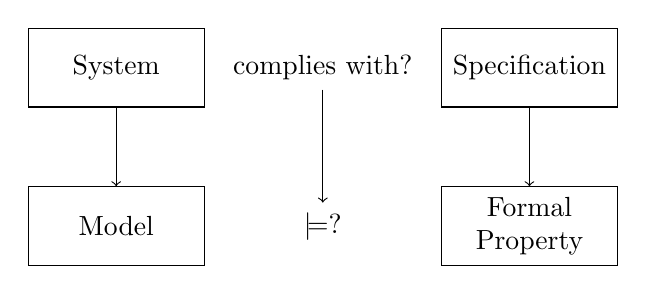
\begin{tikzpicture}
        \tikzstyle{box}=[draw,rectangle,minimum width=2cm,minimum height=1cm,text width=2cm,align=center]
        \node[box] (system) {System};
        \node[box] (specification) [right=3cm of system] {Specification}
            edge[draw=none] node[midway] (comply) {complies with?} (system);

        \node[box] (model) [below=of system] {Model}
            edge[<-] (system);
        \node[box] (properties) [below=of specification] {Formal Property}
            edge[draw=none] node[midway] (models) {$ \models $?} (model)
            edge[<-] (specification);

        \draw[->] (comply) to (models);
    \end{tikzpicture}
    \caption{Overview on Model Checking}
    \label{fig:model-checking}
\end{figure}

\subsubsection{SPIN}
\label{sec:spin}

\gls{spin} (which stands for \textit{S}imple \textit{P}romela \textit{IN}terpreter) is a model checker which has been originally developed by Bell Labs and has been made freely available since the nineties.
As its name already suggests, it uses \gls{promela} as input language.
\textit{The Spin Model Checker: Primer and Reference Manual} which has been used as source for this section, describes \gls{spin} initially as follows:
\begin{displaycquote}[p.1]{SpinManual}
    \gls{spin} can be used to verify correctness requirements for systems of concurrently executing processes.
    The tool works by thoroughly checking either hand-built or mechanically generated models that capture the essential elements of a distributed systems design.
    If a requirement is not satisfied, \gls{spin} can produce a sample execution of the model to demonstrate this.
\end{displaycquote}

As indicated by the quote, \gls{spin} focusses heavily on the verification of distributed or parallel systems.
This is reflected not only in its input language but also in the way how properties are expressed about models.
For an introduction by example to \gls{promela}, cf. snippet \ref{snpt:spin-exm}.
\gls{promela} relies on describing systems as sets of processes that run in parallel where parallel means that each process can advance its state (generally) independent of other processes\footnote{%
    We added the restriction \textit{generally} to the claim because processes can be set up such that they deliberately wait for other processes to send them a message or set some shared state accordingly.
    However, such mechanisms where processes depend on each other always need to be implemented accordingly.
}.

In snippet \ref{snpt:spin-exm}, two processes of the same type \lstinline{user} are declared in line \ref{ln:proc}.
The idea of this snippet is to implement and verify an algorithm that grants these two processes mutually exclusive access to the critical region spanning lines \ref{ln:crit-start}-\ref{ln:crit-end}.
This is ensured by the assertion in line \ref{ln:assert} since variables in \gls{spin} are always initialized to 0 - if two processes had access to the critical region at the same time, \lstinline{cnt} would become 2 at some point.

The details of the protocol implemented in lines \ref{ln:excl-start}-\ref{ln:excl-end} the purpose of which is to grant mutual exclusive access to the critical region are not relevant for this thesis.
However, this part of code gives you an indication for how models written in \gls{promela} look like.
Besides \lstinline{if} statements and labels similar to those in C (cf. line \ref{ln:label}), \gls{promela} supports \lstinline{do}-loops to control process execution flow.
\lstinline{do}-loops run indefinitely until they are exited manually by a \lstinline{break} statement.

As data types, \gls{promela} knows three categories of them: processes, message channels and data objects.
Data objects comprise atomic data types such as \lstinline{byte}, \lstinline{bool}, \lstinline{int}, etc. as well as complex data type defined by \lstinline{typedef} that define a complex structures that have fields of data objects.
Both atomic data types and complex data types are very close to the data types of C.

\begin{figure}
    \begin{lstlisting}[
        caption={Faulty Mutual Exclusion Algorithm Implemented in \gls{promela} \cite{SpinManual}},
        label={snpt:spin-exm}
    ]
        byte cnt;
        byte x, y, z;

        active [2] proctype user() (*\label{ln:proc}*)
        {
            byte me = _pid + 1;
        again: (*\label{ln:label}*)
            x = me; (*\label{ln:excl-start}*)
            if
            :: (y == 0 || y == me) -> skip
            :: else -> goto again
            fi;

            z = me;
            if
            :: (x == me) -> skip
            :: else -> goto again
            fi;

            y = me;
            if (z = me) -> skip
            :: else -> goto again
            fi; (*\label{ln:excl-end}*)

            cnt++; (*\label{ln:crit-start}*)
            assert(cnt == 1); (*\label{ln:assert}*)
            cnt--; (*\label{ln:crit-end}*)
            goto again
        }
    \end{lstlisting}
\end{figure}

Snippet \ref{snpt:spin-output} shows the output when verifying snippet \ref{snpt:spin-exm} with \gls{spin} where we assume that latter snippet was written into a file called \lstinline{mutex_flaw.pml}.
The lines of the output are structured as follows: at the beginning of each line, you see a step index indicating the progress of all processes, then \lstinline{proc X (NAME)} indicates the process that has made progress by its ID and name.
The rest of the line \lstinline{line X ... [CODE]} shows the code executed by the process along with the corresponding line number in the source file\footnote{%
    In this case, line numbers don't fully align with snippet \ref{snpt:spin-exm} but this is not relevant here.
}.
Notice, how processes 0 and 1 progress completely independent from each other, executing code on a line by line basis where each step of any process counts as a state transition of the whole model.

\begin{figure}
    \begin{lstlisting}[
        caption={\gls{spin} Example Output \cite{SpinManual}},
        label={snpt:spin-output}
    ]
        1:  proc    1 (user) line   5 ... [x = me]
        2:  proc    1 (user) line   8 ... [(((y==0) || (y==me)))]
        3:  proc    1 (user) line  10 ... [z = me]
        4:  proc    1 (user) line  13 ... [((x = me))]
        5:  proc    0 (user) line   5 ... [x = me]
        6:  proc    0 (user) line   8 ... [(((y==0) || (y==me)))]
        7:  proc    1 (user) line  15 ... [y = me]
        8:  proc    1 (user) line  18 ... [((z = me))]
        9:  proc    1 (user) line  22 ... [cnt = cnt+1]
        10: proc    0 (user) line  10 ... [z = me]
        11: proc    0 (user) line  13 ... [((x = me))]
        12: proc    0 (user) line  15 ... [y = me]
        13: proc    0 (user) line  18 ... [((z==me))]
        14: proc    0 (user) line  22 ... [cnt = (cnt+1)]
        spin: line 223 of "mutex_flaw.pml", Error: assertion violated
        spin: text of failed assertion: assert((cnt==1))
        15: proc    0 (user) line  23 ... [assert((cnt==1))]
        spin: trail ends after 15 steps
        # processes: 2
            cnt = 2
            x = 1
            y = 1
            z = 1
        15: proc    1 (user) line  23 "mutex_flaw.pml" (state 20)
        15: proc    0 (user) line  24 "mutex_flaw.pml" (state 21)
        2 processes created
    \end{lstlisting}
\end{figure}

Assertions, however, are not the only way to express properties of \gls{promela} models for \gls{spin}.
Furthermore, there are:
\begin{itemize}
    \item Labels
    \item Never claims
    \item Trace assertions
\end{itemize}

Labels have already been introduced informally along with snippet \ref{snpt:spin-exm}.
To express properties about a model, certain types of labels can be used to give semantics to process state.
For example, you can label a certain part of process code as and end-state that might look like an idling-state to \gls{spin} by default.
% TODO: introduce deadlocks
Idling- and end-states are important to \gls{spin} when it's checking for deadlock-freeness of systems.
By default, if all processes are in an idling-state and wait for some kind of signal, this state is considered to be a deadlock.
However, in some situations it might be perfectly fine for some of the processes to idle in a specific state which should not contribute towards deadlocks.
Labeling parts of code as end-state contributes towards this.

Never claims are processes themselves.
% TODO: introduce LTL
They run like any other process but must not terminate otherwise they're regarded as failure.
This is the most complex way to express properties and in fact falls together with writing LTL properties about a model.
Therefore \gls{spin} also allows to express such never properties in LTL directly via their command line interface.

The last type of properties, trace assertions, solely deal with message passing and therefore are not relevant to this thesis.

For some, it might be obvious at this point why we decided against using \gls{spin} as the model checker of this thesis.
Its focus on verifying distributed and parallel systems is obvious and would make implementing an \gls{isa} in it very hard.
In the \textit{Primer and Reference Manual} for \gls{spin} it is written:
\begin{displaycquote}[p.33]{SpinManual}
    \textins{W}e saw that the emphasis in \gls{promela} models is placed on the coordination and synchronization aspects of a distributed system, and not on its computational aspects. \textelp{}
    The specification language we use for systems verification is therefore deliberately designed to encourage the user to abstract from the purely computational aspects of a design, and to focus on the specification of process interaction at the system level.
\end{displaycquote}

However, the \gls{isa} we will attempt to verify
\begin{enumerate*}[label=\alph*)]
    \item will most likely not include components \enquote{interacting at the system level} and
    \item will be verified on a component level, i.e. computationally as well - even in the case where multiple system level components would be given.
\end{enumerate*}

Furthermore, it is unreasonable to assume that an implementation of instructions of an \gls{isa} could be implemented in a single statement of \gls{promela}.
Yet, this should be the goal as otherwise as shown in snippet \ref{snpt:spin-output} what is regarded as state by \gls{spin} would not fall together with what is regarded as state in an \gls{isa}.
For an \gls{isa}, you typically would consider the \textit{state} of registers and memory to be the state of the \gls{isa} whilst some instruction advances this state.
However, for \gls{spin} more complex state transitions would result in us not being able to differentiate architectural states of the \gls{isa} natively since the process implementing the \gls{isa} would change state on each line of code executed.
This could be circumvented by using the \lstinline{atomic} keyword offered by \gls{promela} which lets you wrap a group of \gls{promela} statements such that they're considered as one atomic statement that advances the process state only by one step.
However, this would lead to a model consisting of one process all of its code being wrapped by one \lstinline{atomic} statement.
This would massively contradict the key idea of \gls{spin} of simple models being \textit{abstracted} from computationally complex code.
In this case, we'd have skipped the whole step of abstracting from some computational model that has distributed components running in parallel.
Not only could this lead to performance issues, it also can be safely assumed that the work for this thesis would be cumbersome and might stumble over obstacles induced by abusing \gls{spin}.

\subsubsection{\muZ{} \& \gls{spacer}}

\muZ{} is a \gls{datalog}-engine that provides querying fixed points with constraints and has been proposed in \cite{Hoder11}.
According to \textit{An Introduction to Database Systems} \cite[p.790ff]{Date00}, \gls{datalog} is a descriptive and querying language that originated in the field of database management systems.
At its core, \gls{datalog} programs are sets of \textit{rules} that combine predicates only using variables and constants to Horn-clauses, i.e. disjunctions with one positive literal at maximum.
For example, consider the following rule $ \pi_0 $ which expresses the transitivity of a predicate $ P $:
\begin{equation*}
    \pi_0 := P(a, b) \land P(b, c) \Rightarrow P(a, c)
\end{equation*}
Such programs are then used to \textit{deduct} facts from the set of rules.
To illustrate what this means, we introduce two other rules.
\begin{align*}
    \pi_1 := & P(0, 1) \Rightarrow \top \\
    \pi_2 := & P(a, b) \Rightarrow P(a + 1, b + 1)
\end{align*}
The \gls{datalog}-program $ \Pi := \{ \pi_0, \pi_1, \pi_2 \} $ now induces the relation $ < $ on all natural numbers including $ 0 $.
$ \pi_1 $ sets up a start of induction which, stating that $ 0 $ is smaller than $ 1 $ which is generalized for all natural numbers by $ \pi_2 $.

Whether or not this exact \gls{datalog}-program is supported by a given \gls{datalog}-engine depends on the extensions implemented by the respective engine.
Our example relies on an extension for scalar operators since we use the $ + $ operator.

As briefly mentioned, \gls{datalog} also supports queries.
\gls{datalog} queries comprise only one predicate and a special head $ ? $.
\begin{equation*}
    q_0 := P(0, x) \Rightarrow \; ?
\end{equation*}
The result to a query is the set of all values for each variable that make the predicate true.
In this case, the result set would be $ \{ 1, 2, 3, \dots \} $.
If no variables but only constants are given in the query, \gls{datalog} simply determines whether the given predicate can be derived for the given constants.

\muZ{} now is a \gls{datalog}-engine that comes as part of the SMT solver z3 \cite{Moura08} and adds support for expressing Horn-clauses to it.
For example, consider the implementation of the program $ \Pi $ for \muZ{} as depicted in snippet \ref{snpt:muz-exm}.
This example yields \smt{sat} as result when executed, meaning, that \smt{goal} can be derived from the rules at hand.

\begin{figure}
    \begin{lstlisting}[
        language=SMT2,
        caption={Implementation of $ \Pi $ for \muZ{}},
        label={snpt:muz-exm}
    ]
        (declare-var a Int)
        (declare-var b Int)
        (declare-var c Int)

        (declare-rel ge (Int Int))
        (declare-rel goal ())

        (rule (ge 0 1))                     ; pi_1
        (rule (=>   (ge a b)                ; pi_2
                    (ge (+ a 1) (+ b 1))))
        (rule (=>   (and (ge a b) (ge b c)) ; pi_0
                    (ge a c)))

        (rule (=>   (ge 10 15)
                    goal))
        (query goal)
    \end{lstlisting}
\end{figure}

\gls{spacer} \cite{Komuravelli13} is an algorithm that combines two widely implemented approaches of currently available formal verification tools: \gls{2bmc} and \gls{cegar}.
In its implementation, \gls{spacer} uses \muZ{} as a backend.
The paper describes those techniques as follows:
\begin{displaycquote}[p.1f]{Komuravelli13}
    The key idea of \gls{2bmc} is to iteratively construct an under-approximation \textins{(or refinement)} $ U $ of the target program $ P $ by unwinding its transition relation and check whether $ U $ is safe using \gls{bmc}.
    If $ U $ is unsafe, so is $ P $.
    Otherwise, a proof $ \pi_U $ is produced explaining \textit{why} $ U $ is safe.
    Finally, $ \pi_U $ is generalized (if possible) to a safety proof of $ P $.
    \textelp{}

    Thea idea of \textins{\gls{cegar}} is to iteratively construct, verify, and refine an abstraction (\textit{i.e.}, an over-approximation) of $ P $ based on abstract counterexamples.
\end{displaycquote}

The key to understand how \gls{spacer} works is to understand what under- or over-approximation of programs are.
For the sake of brevity, consider the program $ P $ as depicted in snippet \ref{snpt:spacer-p}.
$ P $ performs an integer division with remainder for a natural number \lstinline{n} by a divisor \lstinline{div} storing the results in \lstinline{ratio} and \lstinline{mod}.
Intuitively speaking, $ \hat{P} $ is an under-approximation (or abstraction) of $ P $ if for every part of $ P $ there is a corresponding part of $ \hat{P} $ whose effects are logically entailed by the original part.
On the other hand, $ P $ is an over-approximation of $ \hat{P} $.
An example for an over-approximation of $ P $ in snippet \ref{snpt:over-p} and an example for an under-approximation of in snippet \ref{snpt:under-p}.
For abstracting $ P $ to $ \hat{P} $ a couple of lines were removed whilst all other were left untouched.

\begin{figure}
    \centering
    \begin{minipage}{.45\linewidth}
        \begin{lstlisting}[
            linewidth=0.9\linewidth,
            caption={Program $ P $},
            label={snpt:spacer-p}
        ]
            n = abs(input());
            div = abs(input());
            ratio = 0;
            mod = 0;
            n = n - div;
            while (0 <= n) {
                ratio++;
                n = n - div;
            }
            mod = div + n;
        \end{lstlisting}
    \end{minipage}

    \begin{minipage}[t]{.45\linewidth}
        \begin{lstlisting}[
            linewidth=0.9\linewidth,
            caption={Refinement $ \bar{P} $},
            label={snpt:under-p}
        ]
            n = abs(input());
            div = abs(input());
            ratio = 0;
            mod = 0;
            n = n - div;
            if (0 <= n) {
                ratio++;
                n = n - div;
                if (0 <= n) {
                    (*\dots*)
                }
            }
        \end{lstlisting}
    \end{minipage}\hspace{0.1\linewidth}%
    \begin{minipage}[t]{.45\linewidth}
        \begin{lstlisting}[
            linewidth=0.9\linewidth,
            caption={Abstraction $ \hat{P} $},
            label={snpt:over-p},
            showlines=true
        ]
        n = abs(input());
        div = abs(input());
        ratio = 0;
        mod = 0;

        while (0 <= n) {

            n = n - div;
        }

        \end{lstlisting}
    \end{minipage}
\end{figure}

With this example at hand it can more easily be seen how \gls{2bmc} and \gls{cegar} relate to under- and over-approximations respectively.
Assume that we want to prove that always \lstinline{0 <= ratio}.
In the case of the refinement $ \bar{P} $ in snippet \ref{snpt:under-p} we could follow the idea of \gls{2bmc} and iteratively check whether \lstinline{0 <= ratio} for finite traces of $ P $.
If a counterexample is found in $ \bar{P} $ it is obvious that this counterexample must also apply to $ P $.
However, if no counterexample is found but a proof for the property at hand can be constructed one can only hope that this proof can be generalized to $ P $.

On the other hand, the converse holds for over-approximations, i.e. abstractions.
If a property is checked for the abstraction $ \hat{P} $ of $ P $ and a positive result in form of a correctness proof is given this proof will apply to $ P $ as well.
However, when a counterexample is given, it is unclear whether it applies to $ P $.
If the counterexample does not apply to $ P $, the idea of \gls{cegar} \cite{Clark00} is to refine the abstraction at hand in such a way that the counterexample does not apply to it anymore and re-iterate on the verification process.

\gls{spacer} uses both of these techniques to prove safety properties of programs expressed in \gls{datalog} using \muZ{}.
These safety properties are expressed using custom relations in \gls{datalog} such as \smt{goal} in snippet \ref{snpt:muz-exm}.
\gls{spacer} then tries to construct a proof why the property at hand cannot be derived from the axioms of the \gls{datalog} program or it gives a counterexample illustrating a possible weakness of the program.
In theory, \gls{datalog} could be used for the implementation of this thesis.
A single predicate could be used to simulate the architectural state of the instruction set architecture at hand whilst each instruction could be modelled via a separate rule.

However, whereas the limiting factor for \gls{spin} was the modelling language, the limiting factor for \gls{spacer} is the output of the tool.
In case of a property failing to be verified, no counterexamples are given but \gls{spacer} simply outputs there is an trace of the program for which a given property does not hold but without specifying the trace itself.
\muZ{} itself can be configured to give a more detailed result however that would still not include a \textit{trace of derivations}.
For \gls{spacer} or \muZ{} to be usable in the context of this thesis, these tools would need to output a log of variable values or steps taken when applying rules.

\subsubsection{nuXmv}

%!TEX root = ../thesis.tex

\section{An Introduction to RISC-V}
\label{sec:risc-v-intro}

\gls{riscv} was originally presented in the technical report \textit{UCB/EECS-2011-62} by the University of California in May 2011 \cite{RiscVISA-org} and since then has undergone many changes.
\gls{riscv} divides its architectural specification into two volumes: in volume 1 the base user-level \gls{isa} is described which is separated into several modules whereas volume 2 defines the privileged architecture and instruction set but still only is available as a draft.
The privileged architecture is not divided into modules but rather \textit{functional groups} that define certain aspects of privileged computing.
Such groups include for example machine- and supervisor-level \glspl{isa} and the description of a platform level interrupt controller.

% TODO: Add motivation/goals of RISC-V

In this thesis, we work with version 2.2 of volume 1 \cite{RiscVISA} and version 1.1 of volume 2 \cite{RiscVISAP}.
\gls{riscv} understands itself as a highly customizable architecture.
Currently, there are four variants of a base integer instruction set - one of which must be implemented by any \gls{riscv} processor - and 13 of optional extensions.
The base integer instruction sets include instructions for integer arithmetic, memory operations (loads and stores), control transfer (jumps and branches) and platform management (environment calls and status register operations).
The base integer instruction sets mainly differ in the word-size and register number.
To cope with these differences, they also make small adjustments to some functionalities but only introduce slight changes to the instruction set itself.
These four base integer instruction sets are given by:
\begin{description}
    \item[RV32I] Base integer instruction set
    \item[RV32E] Base integer instruction set for embedded computing
    \item[RV64I] Base integer instruction set for a 64-bit architecture
    \item[RV128I] Base integer instruction set for a 128-bit architecture
\end{description}

The \gls{riscv} manual differentiates between standard and non-standard extensions but only introduces standard ones.
A standard extension is meant to be compatible with any other standard extension and should be \textcquote{RiscVISA}{generally useful} whilst non-standard extensions might add support for more niche use-cases and do not need to be compatible with all standard extensions.

The set of functionalities offered by standard extensions begins at quite low level with the probably most mundane being the standard extension for integer multiplication and division.
You can find a list of all standard extensions in table \ref{tbl:rv-exts}.

\begin{table}
    \centering
    \begin{tabular}{| c | l |}
        \hline
        \textbf{M} & Integer multiplication and division \\
        \textbf{A} & Atomic instructions \\
        \textbf{F} & Single-precision floating-point arithmetic \\
        \textbf{D} & Double-precision floating-point arithmetic \\
        \textbf{Q} & Quad-precision floating-point arithmetic \\
        \textbf{L} & Decimal floating-point arithmetic \\
        \textbf{C} & Compressed instructions \\
        \textbf{B} & Bit manipulation \\
        \textbf{J} & Dynamically translated languages \\
        \textbf{T} & Transactional memory \\
        \textbf{P} & Packed-SIMD instructions \\
        \textbf{V} & Vector operations \\
        \textbf{N} & User-level interrupts \\
        \hline
    \end{tabular}
    \caption{All \gls{riscv} standard extensions}
    \label{tbl:rv-exts}
\end{table}

\paragraph{Naming strings}
A subset of the \gls{riscv} \gls{isa} is described by a so called \textcquote{RiscVISA}{\gls{isa} naming string} which is defined as:

\begin{grammar}
    <naming-string> ::= `RV' (`32' | `64' | `128') (`I' | `E') <extensions>
\end{grammar}

An example for a naming string is the very common \gls{isa}-subset RV64IMAFD which officially is abbreviated by RV64G.
This subset includes the integer multiplication and division, user-level interrupts, atomic instructions, single-precision and double-precision floating-point arithmetic extensions.

This section will introduce the core of the \gls{riscv} architecture by shedding light on the base integer instruction set in section \ref{sec:rv-base-int-isa} and the mechanisms of the privileged part of the architecture in \ref{sec:rv-priv-arch}.

\subsection{The Base Integer Instruction Set}
\label{sec:rv-base-int-isa}

A \gls{riscv} core consists of multiple \glspl{hart}.
Each \gls{hart} controls its own registers including a \gls{pc} and is equipped with its own instruction fetch unit.
However, multiple \glspl{hart} share the same memory.

\subsubsection{Registers}
A \gls{hart} might either control 16 or 32 general purpose registers which are named from x0 to x32.
All but the RV32E base instruction sets support 32 general purpose registers whereas the base instruction set aimed at embedded computing only supports 16 general purpose registers.

The first of these general purpose registers is hardwired to zero and might be used as a target register when the result of an instruction is not needed.
This might seem overly restrictive at first glance but having such a dedicated \enquote{sink}-register serves a purpose as hardware can take benefit of this extra knowledge to perform optimizations.
For example, \gls{riscv} defines the pseudo-instruction \gls{nop} as \rv{Addi x0, x0, 0} the semantics of which is: Add the constant value 0 to x0 and store the result in x0.
The intention of which is to \textcquote{RiscVISA}{define a canonical NOP encoding to allow microarchitectural optimizations} which is only possible because the hardware can know that no register will \textit{truly} be read or written so a \gls{nop} might terminate directly without waiting for the \gls{alu} to calculate some values which will never be used.

In \gls{riscv}, there is no dedicated \gls{lr} or \gls{sp}.
Instead, it is the obligation of the software to implement certain calling conventions.
Both jump instructions of \gls{riscv}, \gls{jal} and \gls{jalr}, receive a general purpose register as argument to which they store the return address of the respective jump which - in practice - will be the \gls{lr}.

\gls{riscv} supports up to 4096 \glspl{csr} for additional state.
On the user-level without any extension, there are no \glspl{csr} present so we will postpone a more detailed introduction to \glspl{csr} to section \ref{sec:rv-priv-arch} where we have a look at the privileged architecture of \gls{riscv}.

\subsubsection{Instructions}

\paragraph{Integer arithmetic and Boolean instructions}
The base integer instruction set provides instructions for plus and minus, integer comparisons and the Boolean operators AND, OR and XOR.
Most of these instructions are implemented in two version: a register version (or R-type instruction) and an immediate version (or I-type instruction).
In the first case the two operands are given as registers and in the second case one operand is given as register and the other as an immediate value read from memory.
In either case the value is stored in a destination register.

These basic instructions are all side effect free besides from advancing the program counter which means that if the destination register is x0, each of them encodes a no-operation instruction.
This property makes them particularly easy to analyze.
However, as a side-effect, this means that there is no built-in support for overflow checks via flags in some dedicated \gls{csr}.
There also is no special instruction to handle this.
The authors of the manual show that in general, overflow checks for addition can be handled with three additional instructions after an add instruction:

\begin{lstlisting}[language=rv,caption={General overflow checking \cite{RiscVISA}},label={snpt:rv-overflow}]
Add  t0, t1, t2          # Set R[t0] to R[t1] + R[t2]
Slti t3, t2, 0           # Set R[t3] to R[t2] < 0
Slt  t4, t0, t1          # Set R[t4] to R[t0] < R[t1]
Bne  t3, t4, overflow    # If R[t3] != R[t4] branch to overflow
\end{lstlisting}

The gist of snippet \ref{snpt:rv-overflow} boils down to: we can check if there was overflow when calculating $ a + b $ by checking whether $ b < 0 \leftrightarrow a + b < a $ is false, i.e. \textcquote{RiscVISA}{the sum should be less than one of the operands if and only if the other operand is negative}.

\paragraph{Memory operations}
There are two types of instructions that deal with external memory.
Firstly, simple load and store instructions that read from or write to memory.
Secondly, FENCE instructions that synchronize memory access between multiple \glspl{hart}.

Memory in \gls{riscv} is byte-addressable.
Therefore, load and store operations in \gls{riscv} can read or write words of size 8-, 16-, 32-, 64- or 128-bits, depending on the maximum word length of the base instruction set of choice.
Read- and write-addresses don't have to be aligned by software before using them, however, if they are not, the architecture must first align them before fetching from or storing to them, i.e. reading a 32-bit word from memory at address 0x1 is impossible.
If this address is given as argument to a respective load instruction it'll be aligned to the address 0x0.

\paragraph{Control transfer instructions}
There are two types of instructions that can control program flow in \gls{riscv}: jumps and branches.
In short, jumps are performed unconditionally and can target a wider range in memory (at least $ \pm 2^{20}\text{bits} $ in case of a 32-bit architecture) whereas branches are performed conditionally, only can target a narrower range in memory ($ \pm 2^{12}\text{bits} $ in case of a 32-bit architecture) and always must branch to \gls{pc}-relative addresses.

In contrast to memory operations, addresses targeted by jumps must be aligned correctly otherwise an exception will be generated.

Jumps are intended to call routines and functions.
This is why they store a return address to some general purpose register.
Branches on the other hand are intended to control the program flow of one such routine or function, e.g. to implement an \textit{if-else} structure or \textit{for}-loops where code won't return from the branched execution.
\gls{riscv} is agnostic about the details of calling conventions for routines, e.g. how the stack is organized, which general purpose registers are used as \gls{lr} or \gls{sp}, and leaves these details to be implemented by software running on the core.

\paragraph{Platform management instructions}
The last type of instructions we will have a look at are platform management instructions.
The \gls{riscv} manual also knows this category and divides it into two subcategories: instructions that deal with \glspl{csr} and other instructions that perform operations that potentially need some form of privilege.
Examples for the former category are straight forward.
\gls{riscv} knows instructions to read or write complete \glspl{csr} but also knows operations to modify single bits only.
For the latter category, \gls{riscv} only knows two instructions at the base instruction set level which are \gls{ecall} and \gls{ebreak} instructions.
We will inspect these instructions in more detail in section \ref{sec:rv-priv-arch}.

\paragraph{Summary}
The base integer instruction set of \gls{riscv} gives you everything you need for implementing a comfortable Turing-machine but pretty much nothing more.
You can perform basic arithmetic with integers or bit vectors of Booleans, load and store results of your calculations and abstract your code by using jumps and branches.
At this point, there is no state with predefined semantics, i.e. all state available is given by storage that can only influence computation when used by a programmer.

Only the platform management instructions give a hint on the complexity that is offered by the \gls{riscv} architecture to allow abstracting processing done on the core.

\subsection{The Privileged Architecture}
\label{sec:rv-priv-arch}

The privileged architecture of \gls{riscv} in \cite{RiscVISAP} mainly specifies three concepts:
\begin{enumerate}
    \item Three levels of privilege
    \item Exceptions, traps and interrupts
    \item Memory attributes
\end{enumerate}

The three levels of privilege form the basis of everything that is defined by the privileged architecture.
The purpose of interrupts and exceptions is not only to handle error conditions that arise during runtime but also to communicate between privilege layers.
Therefore, interrupts and exceptions are being used by up to this point unmentioned auxiliary mechanisms of the architecture that aid the highest privilege in administrating the platform.

Also, memory attributes rely on these levels of privilege as they define which mode is eligible to do some operation on some region of memory.

In this section, we will subsequently introduce the aforementioned concepts and conclude with a sketch of the auxiliary mechanisms that build on top of these.

\subsubsection{Levels of Privilege}

\gls{riscv} knows three privilege levels: user-mode, supervisor-mode and machine-mode\footnote{%
    In an earlier version, there was a fourth privilege-mode being hypervisor-mode that sat between supervisor- and machine-mode.
    However, support for this mode has been dropped.
    This leads \gls{riscv} still with the need to encode mode-relative bit-fields in a size of 2 where 00 stands for user-, 01 for supervisor and 11 for machine-mode.
    10 is reserved in most places.
}.
Each implementation of the \gls{riscv} specification must at least provide machine-mode as a base mode of operation.
Besides this, there are two other choices of privilege levels netting in three different configurations:
\begin{enumerate}
    \item Machine-mode only as a \textcquote{RiscVISA}{simple embedded system}
    \item User and machine-mode as a \textcquote{RiscVISA}{secure embedded system}
    \item User, supervisor and machine-mode as a \textcquote{RiscVISA}{\textins{system} running Unix-like operating systems}
\end{enumerate}

A visualization of these three combinations is given in figure \ref{fig:rv-priv-lvls} where they are depicted from left to right.
A simple embedded system might be the cheapest to implement and manufacture, however, this system lacks any protection against malicious application code, i.e. one would only want to run such a system in very basic scenarios where full control over all source code and the device itself can be guaranteed.

A secure embedded system supports some application to be run on it while an \gls{aee} running in machine-mode controls the execution of this application.
The application communicates to the \gls{aee} via an \gls{abi} that defines the possible interactions between an application and an \gls{aee}.

A system running a Unix-like \gls{os} enhances on this by having an \gls{os} running in supervisor-mode that communicates with multiple applications running in parallel via an \gls{abi} and itself is managed by a \gls{see} which communicates with the \gls{os} via a \gls{sbi}.
The \gls{see} runs in machine-mode.

\begin{figure}
    \centering
    \subcaptionbox{\centering Simple embedded system}
    [0.18\textwidth]{
        \begin{tabular}{| c |}
            \hline
            Application \\ \hline
        \end{tabular}
    }
    \quad
    \subcaptionbox{\centering Secure embedded system}
    [0.18\textwidth]{
        \begin{tabular}{|c|}
            \hline
            Application \\ \hline
            \cellcolor{black} \textcolor{white}{ABI} \\ \hline
            AEE \\ \hline
        \end{tabular}
    }
    \quad
    \subcaptionbox{\centering System with Unix-like OS}
    {
        \begin{tabular}{| c | c | c |}
            \cline{1-1} \cline{3-3}
            Application & \multirow{2}{*}{\dots} & Application \\
            \cline{1-1} \cline{3-3}
            \cellcolor{black} \textcolor{white}{ABI} & & \cellcolor{black} \textcolor{white}{ABI} \\ \hline
            \multicolumn{3}{| c |}{OS} \\ \hline
            \multicolumn{3}{| c |}{\cellcolor{black} \textcolor{white}{SBI}} \\ \hline
            \multicolumn{3}{| c |}{SEE} \\ \hline
        \end{tabular}
    }
    \caption{Privilege level combinations \cite{RiscVISA}}
    \label{fig:rv-priv-lvls}
\end{figure}

To keep things simple, we will focus on secure embedded systems in this thesis\footnote{%
    This will be justified in more detail in section \ref{sec:model} where we introduce the model that will be verified as part of this thesis.
}.
This means that the architecture we will be working with supports two modes: user- and machine-mode.
Machine-, user- and supervisor-mode do not simply form a linear order of privilege attributes of code execution.
They differ in the concepts that are available to them and therefore must be handled separately.
However, as we will focus on secure embedded systems, we will leave out many parts of the specification which are about supervisor solely.
Supervisor-mode will be handled wherever it fits in the bigger picture but not on its own.

\subsubsection{Exceptions, traps and interrupts}
\label{sec:rv-exn}

Volume 1 of the specification introduces the concept of exceptions, traps and interrupts as follows:
\begin{displaycquote}{RiscVISA}
    We use the term \textit{exception} to refer to an unusual condition occurring at run time associated with an instruction in the current RISC-V thread.
    We use the term \textit{trap} to refer to the synchronous transfer of control to a trap handler caused by an exceptional condition occurring within a RISC-V thread.
    Trap handlers usually execute in a more privileged environment.

    We use the term \textit{interrupt} to refer to an external event that occurs asynchronously to the current RISC-V thread.
    When an interrupt that must be serviced occurs, some instruction is selected to receive an interrupt exception and subsequently experiences a trap.

    The instruction descriptions in following chapters describe conditions that raise an exception during execution.
    Whether and how these are converted into traps is dependent on the execution environment, though the expectation is that most environments will take a \textit{precise} trap when an exception is signaled \textelp{}.
\end{displaycquote}

This - in short - means that a trigger-hierarchy for interrupts, traps and exceptions can be recognized which is depicted in figure \ref{fig:trigger-hierarch}.
In general, interrupts occur asynchronously and trigger synchronous exceptions to be generated for a \gls{hart} which in turn may generate traps but also might be handled otherwise.
The specification mentions the example of the floating-point extension in which exceptions not necessarily generate traps.

\begin{figure}
    \centering
    \tikz \graph[grow right sep] {
        Interrupt -> Exception -> {Trap, ?};
    };
    \caption{Trap-Trigger-Hierarchy}
    \label{fig:trigger-hierarch}
\end{figure}

For the sake of simplicity, we will assume that every exception causes a trap.
As we will not implement any floating-point arithmetic extension, the specification does not demand from us to handle exceptions otherwise and doing so does not serve any purpose at this point.
In following paragraphs, we will give an introduction to the control flow of dealing with interrupts which is depicted in figure \ref{fig:interrupt-handling} and follows these steps:
\begin{enumerate}
    \item If an interrupt or exception is pending, determine the privilege mode to take the trap
    \item Check if the interrupt is enabled
    \item Take the trap
    \item Return from trap handler
\end{enumerate}
Interrupt handling can be understood as a generalized form of exception handling as exception handling in principle works the same but has fewer steps.

\begin{figure}
    \centering
    \begin{tikzpicture}[node distance = 1.5cm, auto]
        \node[block] (pending) {
            An interrupt $ i $ is pending in mode $ y $; let $ x := \text{machine-mode} $
        };

        \node[decision] (takePre) [below=of pending] {$ x\text{ideleg}[i] $ and $ x > y $?};
        \path[line] (pending) -- node[midway] (p2tp) {} (takePre);

        \node[block,text width=8em] (deleg) [left=of takePre] {$ x := x - 1 $};

        \path[line] (takePre) -- node[near start] {yes} (deleg);
        \path[line] (deleg) |- (p2tp);

        \node[decision] (takePre2) [right=of takePre] {$ x > y $ or $ x = y $, $ x\text{status}.x\text{IE} $, $ x\text{ie}[i] $?};
        \path[line] (takePre) -- node[near start] {no} (takePre2);

        \node[block,text width=16em] (take) [below=of takePre2] {
            Write $ x\text{tval} $ accordingly and let $ t := x\text{tvec} $, furthermore set:\\
            $ \begin{aligned}
                & x \text{status}.x\text{PP} := y \\
                & x \text{status}.x\text{PIE} := x\text{status}.x\text{IE} \\
                & x\text{status}.x\text{IE} := 0 \\
                & x\text{epc} := \text{current address} \\
                & x\text{cause}[31] := 1 \\
                & x\text{cause}[30..0] := i \\
            \end{aligned} $
        };
        \path[line] (takePre2) -- node[near start] {yes} (take);
        \path[line,dashed] (takePre2.east) -- node[near start] {no} ++(right:1.5cm);

        \node[decision,text width=6.5em] (jumpPre) [left=of take] {$ x\text{tvec.MODE} $?};

        \path[line] (take) -- (jumpPre);

        \node[block,text width=8em] (vectored) [left=of jumpPre] {$t := t + 4 \times i $};
        \path[line] (jumpPre) -- node[near start] {yes} (vectored);

        \node[block] (handling) [below=of jumpPre] {Jump to $ t $ and execute instructions};
        \path[line] (jumpPre) -- node[near start] {no} node[midway] (jp2h) {} (handling);
        \path[line] (vectored) |- (jp2h);

        \node[block] (return) [below=of handling] {
            Set privilege mode to $ x\text{status}.x\text{PP} $ and $ x\text{status}.x\text{IE} $ to $ x\text{status}.x\text{PIE} $, then jump to $ x\text{epc} $
        };
        \path[line] (handling) -- node[near start] {on $ x\text{RET} $} (return);
    \end{tikzpicture}
    \caption{Interrupt handling flow-chart}
    \label{fig:interrupt-handling}
\end{figure}

\paragraph{Interrupt and exception handling}
There are three categories of interrupts: external interrupts, timer interrupts and software interrupts.
External interrupts are used to signal exceptional events occurring on some external device that is connected to the core.
Timer interrupts can be used to track time.
Code can use certain \glspl{csr} to signal to the platform that it needs to be alerted when a given amount of real world time has passed.
Such an alert will be given by a timer interrupt.
More on this in section \ref{sec:other-mechs}.
Software interrupts can be set pending by software running on the same \gls{hart} with equal or higher privilege than the targeted privilege mode.
Software interrupts have no predefined semantics and thus can be used by programmers or system designers in every imaginable way.

Each of these categories of interrupts can target any privilege-mode netting a total of 6 interrupts available to the platform in our case (or 9 if supervisor-mode is supported).
These interrupt-types are associated with indices in the range from $ 0_{10} $ to $ 11_{10} $, also called interrupt code\footnote{%
    The reader might have noticed that these are more indices than needed to encode all interrupts available - even if supervisor-mode is present.
    Indices 2, 6 and 10 currently are reserved because support for hypervisor-mode was dropped.
    The two least significant bits of the interrupt indices correspond to their respective mode thus 2, 6 and 10 are reserved as their two least significant bits are 10 corresponding to hypervisor-mode.
}.
An overview of all interrupt codes can be found in table \ref{tbl:interrupt-exception-codes}.
Interrupts can be set pending individually in the \gls{mip} register.
An interrupt is set pending if the bit corresponding the interrupts index is set to 1.

If an interrupt or exception is pending, it must first be decided which privilege mode should take the trap to handle the exception generated.
By default, all interrupts and exceptions will be handled by machine-mode.
However, interrupts and exceptions can be delegated to less privileged modes via the \gls{mideleg} and \gls{medeleg} register\footnote{%
    It would also be possible to delegate traps by using the \gls{mret} instruction and setting all corresponding \glspl{csr} accordingly.
    However, this would come with a higher latency as a couple of jumps would need to be performed first.
}.
Similar to \gls{mip} and \gls{mie}, each bit field of \gls{mideleg} corresponds to the interrupt of the same index.
Exceptions also have an exception code assigned and thus, fields of \gls{medeleg} correspond to these codes.
An interrupt or exception can only be delegated to modes equally or higher privileged than the mode the interrupt or exception was targeting originally for example, if an interrupt is targeting supervisor-mode it must be handled by machine-mode or can optionally be delegated to supervisor-mode.
If an interrupt is delegated to mode $ x $, the corresponding bit in $ x\text{ip} $ reads accordingly and $ x\text{ie} $ becomes writable otherwise both registers appear to be hardwired to zero.

After the mode to be targeted by the trap has been determined, it must be checked whether the given interrupt is actually enabled.
Exceptions can't be disabled and therefore will always be taken - as a consequence the following checks will be omitted for exceptions.
Interrupts on the other hand can be dis- or enabled individually in the \gls{mie} register.
Analogously to the \gls{mip} register, an interrupt is enabled if the bit corresponding the interrupts index is set to 1.
Additionally, there is the \gls{mstatus} register which can globally dis- or enable interrupt handling for a specific mode via its $ x\text{IE} $ bits ($ x \in \{ \text{M}, \text{S}, \text{U}\} $\footnote{%
    In future, we will simply use $ x $ or other variables as placeholders for a mode-flag without specifically introducing the variable.
}).
The \gls{ustatus} register only is a restricted view on \gls{mstatus} and therefore \gls{mstatus} holds these bits not only for machine- but any mode.
These $ x\text{IE} $ fields, however, are only taken into account if the \gls{hart} operates at an equal or higher privilege mode than targeted, i.e. interrupts are always enabled globally it is targeting a mode of higher privilege than current operation.
Finally, an interrupt will be taken if interrupts are globally enabled \textit{and} the interrupt itself is enabled in the \gls{mie} register.

If a pending interrupt is taken, the \gls{mepc}, \gls{mcause} and \gls{mtval} registers are written and the platform will jump to a base address held by the \gls{mtvec} register.
\gls{mtvec} also holds a field that controls whether interrupts can be \textit{vectored}, i.e. for interrupts the \gls{pc} is not set to the base address for handling trap but to $ \text{base} + 4 \times \text{cause} $.
\gls{mepc} holds the address of the original instruction stream that was preempted, i.e. either the address of the instruction that caused the exception or the instruction that was next to be executed as a external interrupt was taken.
\gls{mcause} holds an identifier of the current interrupt or exception being handled by the trap.
The most significant bit indicates whether an interrupt is currently being served and all other bits hold the exception or interrupt code.
\gls{mtval} serves as a register to hold arguments for a trap handler.
Technically, it holds \textcquote{RiscVISAP}{exception-specific information to assist software in handling the trap}.
One example for such \enquote{exception-specific information} is that \gls{mtval} can contain the faulting bits of an instruction for an illegal instruction exception whereas \gls{mepc} would only point to the instruction in memory as a whole therefore giving no specific information about which part of the instruction caused the exception.

\gls{mstatus} also holds bits to \enquote{stack} certain values when handling exceptions or interrupts.
Nested interrupts are only supported between privilege modes.
On a trap to handle an interrupt in mode $ x $, interrupts are disabled and the value of the interrupt-enable bit is \enquote{stacked} into a prior-interrupt-enable bit $x\text{PIE} $, i.e. $ x\text{PIE} := x\text{IE} $ and $ x\text{IE} := 0 $.
Additionally, there is a prior-privilege bit $ x\text{PP} $ that stores the privilege mode before the trap was taken.

% TODO: Maybe exactly one instruction? How does alignment play into this?
Note that due to the small offset between vectored interrupt jump destinations, the instructions located there can't perform much more than jumping to the \textit{real} trap handler.
Furthermore, as exceptions can't be vectored, any differentiation between those must be performed by software.

\begin{table}
    \centering
    \begin{tabular}{| r | r | l |}
        \hline
        Interrupt & Exception Code & Description \\
        \hline
        1 & 0 & User software interrupt \\
        1 & 1 & Supervisor software interrupt \\
        1 & 2 & \textit{Reserved} \\
        1 & 3 & Machine software interrupt \\
        \hline
        1 & 4 & User timer interrupt \\
        1 & 5 & Supervisor timer interrupt \\
        1 & 6 & \textit{Reserved} \\
        1 & 7 & Machine timer interrupt \\
        \hline
        1 & 8 & User external interrupt \\
        1 & 9 & Supervisor external interrupt \\
        1 & 10 & \textit{Reserved} \\
        1 & 11 & Machine external interrupt \\
        \hline
        1 & $ \geq $ 12 & \textit{Reserved} \\
        \hline
        0 & 0 & Instruction address misaligned \\
        0 & 1 & Instruction access fault \\
        0 & 2 & Illegal instruction \\
        0 & 3 & Breakpoint \\
        0 & 4 & Load address misaligned \\
        0 & 5 & Load access fault \\
        0 & 6 & Store \textelp{} address misaligned \\
        0 & 7 & Store \textelp{} access fault \\
        0 & 8 & Environment call from U-mode \\
        0 & 9 & Environment call from S-mode \\
        0 & 10 & \textit{Reserved} \\
        0 & 11 & Environment call from M-mode \\
        0 & 12 & Instruction page fault \\
        0 & 13 & Load page fault \\
        0 & 14 & \textit{Reserved} \\
        0 & 15 & Store \textelp{} page fault \\
        0 & $ \geq $ 16 & \textit{Reserved} \\
        \hline
    \end{tabular}
    \caption{Interrupt and exception codes \cite{RiscVISAP}}
    \label{tbl:interrupt-exception-codes}
\end{table}

\paragraph{Summary}
You can find an overview over all registers that are involved in trap handling in table \ref{tbl:trap-csrs}.
Those \glspl{csr} which are available to user-mode would also be available to supervisor-mode in this context.
Registers written in italic font are not actual registers on their own but provide a restricted view on their respective machine-mode counterparts.

\begin{table}
    \centering
    \begin{tabular}{| c c || l |}
        \hline
        \textbf{Machine-mode} & \textbf{User-mode} & \textbf{Description} \\
        \acrshort{mstatus} & \textit{\acrshort{ustatus}} & Status \\
        \acrshort{mie} & \textit{\acrshort{uie}} & Interrupt enable \\
        \acrshort{mip} & \textit{\acrshort{uip}} & Interrupt pending \\
        \acrshort{mtvec} & \acrshort{utvec} & Trap-vector base address \\
        \acrshort{mscratch} & \acrshort{uscratch} & Scratch \\
        \acrshort{mepc} & \acrshort{uepc} & Exception program counter \\
        \acrshort{mcause} & \acrshort{ucause} & Trap cause \\
        \acrshort{mtval} & \acrshort{utval} & Trap value \\
        \acrshort{medeleg} & & Exception delegation \\
        \acrshort{mideleg} & & Interrupt delegation \\
        \hline
    \end{tabular}
    \caption{Trap-handling \glspl{csr}}
    \label{tbl:trap-csrs}
\end{table}

To summarize the mechanisms that play into interrupt and exception handling, recall the four steps to interrupt and exception handling we introduced at the beginning of this section.
These can now be filled with more details:
\begin{enumerate}
    \item If an interrupt or exception is pending, determine the privilege mode to take the trap by checking the targeted privilege mode and any delegation settings
    \item If an interrupt is pending, check that interrupts are enabled globally and the specific interrupt is enabled as well
    \item Take the trap by jumping to to trap base vector and if an interrupt is being serviced take vectoring into account
    \item Return from trap handler
\end{enumerate}

The differences between handling exceptions and interrupts can be summarized by the following:
\begin{itemize}
    \item Exception can't be disabled therefore they will always be handled
    \item $ x\text{cause}[31] $ is written with $ 0 $
    \item Exceptions can't be vectored therefore the \gls{pc} will always be set to $ x\text{tvec} $
\end{itemize}

One would need to alter figure \ref{fig:interrupt-handling} by replacing most interrupt-related \glspl{csr} with their exception-related counterpart if possible.
An exception to this is $ x\text{status}.x\text{IE} $ which still is set to 0 meaning that it is not possible to preempt handling an exception by handling an interrupt.

Finally, note that exceptions are handled as soon as they occur.
This is necessary as exceptions always are closely related to the current stream of instructions and therefore need attention before said stream can continue to be executed.
The only exception to this are other interrupts which are handled before any exception with the following decreasing order of priority: external interrupts, software interrupts, timer interrupts, exceptions.
% Source: https://stackoverflow.com/a/56402079/7194995
\gls{riscv} knows no concept of settings exceptions pending, this however, isn't necessary.
If an exception occurs while an interrupt is set pending, the interrupt can be handled with \gls{mepc} being set to the address of the faulting instruction which either will again fault after the interrupt has been handled or will succeed by some magical condition in which case it does need any further attention.

% TODO: Mention what I didn't mention; e.g. specific parts of mstatus

\subsubsection{Memory Attributes}
\label{sec:memory-attrs}

In the previous paragraph, we mentioned that \gls{mstatus} contains some bits that are not directly relevant to trap handling.
Alongside these bits we will introduce another \gls{csr} that is related to trap handling but not directly necessary in this section.

These two remaining fields of \gls{mstatus} deal with memory privilege translation for machine-mode.
Firstly, there is the MPRV bit which can translate memory access privilege.
This bit is only available if at least two privilege modes are supported otherwise it is hardwired to zero.
If MPRV is set to one, \textcquote{RiscVISAP}{load and store memory addresses are translated and protected as though the current privilege mode were set to MPP}, i.e. they're performed with the privilege level that has was preempted by taking the trap.
Secondly, there is the MXR field that allows to read executable memory regions.
If MXR is not set, attempting to read from a memory region marked as executable will fail.
If MXR is set, such reads can succeed if said region is also marked as readable.
% TODO: is page-based virtual memory given?
MXR is only applicable though, if page-based virtual memory is in place.

The last register we will introduce is the \gls{mscratch} register which can be used by machine-mode to be read and written to for preserving any value the machine-mode would like to see preserved.
The intended use-case for this register by the specification is that \textcquote{RiscVISAP}{it is used to hold a pointer to a machine-mode \gls{hart}-local context space and swapped with a user register upon entry to a \textins{machine}-mode trap handler}.

% TODO: Introduce pma- and pmpcfg

\subsubsection{Other Mechanisms}
\label{sec:other-mechs}

\paragraph{Timer and performance counter \glspl{csr}}
There also is a group of registers dealing with timers and hardware performance monitoring, namely: \gls{mtime}, \gls{mtimecmp}, \gls{mcycle}, \gls{minstret}, \gls{mhpmcountern}, \gls{mhpmeventn} and \gls{mcounteren} but we won't go into detail here as we will be ignoring these registers as well.
The reasoning for skipping these is not as straight-forward as for the previously introduced registers.
In general, timer and performance counting registers can be used for side channel attacks.
In \cite{Qian16} the authors give an overview over timing-side-channel-attacks which by their very nature always need to rely on some notion of time.
This notion can be given by timer and performance counter registers which for example hold the number of instructions executed since a given point in time.
For example, the authors discuss an attack where a side channel to OpenSSL's implementation of \gls{rsa} could be introduced by differentiating between multiplications and squares being performed.
Such a differentiation could be easily done if performance counter registers where to count such instructions and were to leak information to lower privilege levels.
This means that in principle, timer and performance counter registers are relevant for the security of an architecture.
However, we find that they do not introduce new notions of information flow to the architecture and are therefore redundant to our thesis.

It is the case that contents of these registers are confidential as their contents might be used to introduce side-channels to other applications running on the processor.
However, their core mechanisms are not unique.
They can be read and written to and might generate interrupts but this is nothing new to the architecture.
We therefore think that dealing with information flow in general is sufficient for our approach and will ignore these registers.

Besides the interrupts and exceptions that have been introduced in the last few paragraphs, there are two further \textit{exceptional conditions} that can occur in a \gls{hart}.

\paragraph{Reset}
The first of these is the reset.
The specification does not explicitly define how resets are triggered but it is clear that resets must be triggered by hardware at least., e.g. by the push of a button that is on a shared board with the processor.
As the specification gave an exhaustive list of exceptions and interrupts available to the system in table \ref{tbl:interrupt-exception-codes} we assume here that resets can be triggered by hardware only.

On reset, the \gls{pc} is set to an implementation defined address, the privilege mode is set to machine-mode, the MIE and MPRV bits in \gls{mstatus} are set to 0 and \gls{mcause} should be written with implementation-defined values to indicate the cause of the reset.
The specification explicitly mentions that \textcquote{RiscVISAP}{%
    \textins{a}ll other hart state is undefined
} although software located at the reset vector might write \glspl{csr} with arbitrary values.

% Source: https://stackoverflow.com/a/46989066/7194995
Although the specification itself says that the \textcquote{RiscVISAP}{\texttt{pc} is set to an implementation-defined reset vector} and does not lay any constraints on this, we think that this address must not be the same as \gls{mtvec}.
The reason for this is given in a comment to this section where it says:
\begin{displaycquote}{RiscVISAP}
    \texttt{mcause} reset values may alias \texttt{mcause} values following synchronous exceptions.
    There is no ambiguity in this overlap, since on reset the \texttt{pc} is set to a different value than on other traps.
\end{displaycquote}

Although comments should not be taken with the same weight as regular passages of the specification, the intent behind this comment is quite clear and as it only slightly contradicts the specification we will go with this interpretation.

\paragraph{Non-Maskable Interrupts}
The other exceptional condition are \glspl{nmi}.
The specification describes these as: \textcquote{RiscVISAP}{%
    \textins{NMIs} are only used for hardware error conditions, and cause an immediate jump to an implementation-defined NMI vector running in M-mode regardless of the state of a hart's interrupt enable bits.
}
Similar to resets, nothing is said about the mechanisms to trigger \glspl{nmi} in the specification.
For the same reasons given in the paragraph about reset, we will assume that \glspl{nmi} can only be triggered by hardware.

On jump to the \gls{nmi} handler address, \gls{mepc} is written with the next address to be read and executed and \gls{mcause} is written with information about the cause of the \gls{nmi}.
Other \glspl{csr} are left untouched.

% TODO: Summarize

%!TEX root = ../thesis.tex

\section{Information Flow Control}

% TODO: Introduction

\subsection{Information Flow Semantics for Instructions}
\label{sec:ifc-model}

% TODO: reference to introduction of Ferraiuolo17 paper

% 1. Introduce Ferraiuolo17 type system rules (only relevant ones)
% 2. Transform lattice transitions to two independent labelings with sup and inf operation
% 3. Introduce defaults
% 4. Translate transitions

% TODO: ensure that this introduction is free of redundancies
In \cite{Ferraiuolo17} the authors introduce an extension to the \gls{hdl} SecVerilog in form of a type system that implements static information flow control forming the new language SecVerilogBL.
They evaluated their approach by successfully finding some known bugs in the Arm architecture.
% TODO: evaluate their results more strongly and compare them to mine
Their approach includes two key ideas:
\begin{enumerate}
    % TODO: "that annotate information" is too broad
    \item A lattice of security labels that annotate information
    \item A type system that allows them to statically track information through Verilog code
\end{enumerate}
In short, the security labels represent the semantics of pieces of information while the type system rules define how information moves through the \gls{hdl} code.
In this section, we will apply these two ideas to an \gls{isa}.
We will apply the ideas of the type system developed in \cite{Ferraiuolo17} to the semantics of the instructions specified by the \gls{isa} of MINRV8 by giving information flow semantics on a per-instruction basis.
This transformation is necessary because in our practical scenario, we cannot rely on the same computational power as a static type checker can.
In our implementation, we will need to realize the information flow control via state-system-transition rules expressed in propositional logic.

\cite{Ferraiuolo17} introduces four information flow labels $ \Sigma = \{ \PT, \PU, \CT, \CU \} $ which stand for public/trusted, public/untrusted, confidential/trusted and confidential/untrusted.
As you can see, each of these four labels comprises two tokens from two domains of information flow control.
The first of these domains is the one of \textit{confidentiality} - each of the labels states that a piece of information is either public (\P{}) or confidential (\C{}).
The second of these domains is the one of \textit{integrity}, i.e. are the values we deal with integrous or - in other words - not malicious?
Each of the labels states that a piece of information is either trusted (\T{}) or untrusted (\U{}).

These labels have a partial order defined $ \preceq $ on them which induces a supremum $ \sqcup $ and an infimum $ \sqcap $ operator on $ \Sigma $.
This partial order is depicted in figure \ref{fig:sec-lattice} as a hasse diagram.
The intuition behind the ordering is that information is always allowed to flow up in the hasse diagram while it is not allowed to flown down.

\begin{example}
    Remember, that this lattice was defined with a type system in mind.
    For information to flow up in this context is best illustrated with the following code snippet\footnote{%
        The syntax of this snippet is \textit{not} SecVerilogBL.%
    }:
    \begin{lstlisting}
        int a : PT = 0;
        int b : PU = a;
    \end{lstlisting}

    In this example, first a variable called \asl{a} is initialized and labelled with \PT{}.
    Then, the value of \asl{a} is assigned to another newly initialized variable labelled with \PU{}.
    This flow of information would be permitted by the lattice $ (\Sigma, \sqcup, \sqcap) $ as information that is labelled with \PT{} flows to a destination that is labelled with \PU{} which is $ \preceq $-greater than \PT{}.

    However, if this flow of information was to occur the other way round, it would have been prohibited.
\end{example}

\begin{figure}
    \centering
    \begin{tikzpicture}
        \begin{scope}
            \node (pt) {\PT};
            \node[above right=of pt] (ct) {\CT}
                edge (pt);
            \node[above left=of pt] (pu) {\PU}
                edge (pt);
            \node[above right=of pu] (cu) {\CU}
                edge (ct)
                edge (pu);
        \end{scope}
    \end{tikzpicture}
    \caption{Security lattice for SecVerilogBL \cite{Ferraiuolo17}}
    \label{fig:sec-lattice}
\end{figure}

% TODO: Do I need a reference for the sequent calculus?
Of course, there are more complex operations in SecVerilogBL than simply assigning values to variables.
In reaction to that, the authors of \cite{Ferraiuolo17} introduce type system rules to define how information flows throughout the system, i.e. how operations generate new security labelings in the form of types.
Type system rules are written like proofs of sequent calculus.

\begin{example}
    Consider this example of a proof written in sequent calculus:
    \begin{prooftree}
        \AxiomC{$ A $}
        \AxiomC{$ B $}
        \BinaryInfC{$ C $}
    \end{prooftree}

    This proof states that the formula $ C $ can be derived from the formulas $ A $ and $ B $ or more formally that: $ A, B \vdash C $.
\end{example}

In the context of type systems, formulas used in proofs of sequent calculus often are so called \textcquote{Ferraiuolo17}{typing judgements} where some \textit{environment} types some \textit{expression}, e.g. if $ X $ is a type environment, $ x $ an expression and $ \tau $ a type one possible typing judgement would be $ X \vdash x : \tau $ which means that $ x $ is of type $ \tau $ under the environment $ X $.
The authors of \cite{Ferraiuolo17} introduce three environments:

\begin{description}
    \item[Standard environment] $ \Gamma $ maps variables to their respective security labeling type, i.e. a function mapping \texttt{int}s as bit indices to security labels (more on this later).
    % TODO: Why must there be a width environment? Introduce how HDLs look like at the beginning of this passage
    \item[Width environment] $ \W $ maps variables to their respective bit vector length.
    \item[Kind environment] $ \Theta $ allows the lifting of security labels to functions mapping bit indices to security labels and can make type judgements of the form $ \Theta \vdash \tau : \texttt{int} \rightarrow l $ where $ l $ is the type of the security labels and $ \tau $ is a type mapped to by $ \Gamma $.
\end{description}

You can find an overview of those type system rules of \cite{Ferraiuolo17} which are relevant to us in figure \ref{fig:type-rules}.
The most simple type system rule probably is T-Const which types constant expressions $ n $.
% TODO: reflect on why it is sensible to assume that constants are trusted in their scenario but not in ours
These are always of type $ \bot $, i.e. \PT, and of the corresponding width $ w $.
The other type system rules share a pattern.
They assume one or two expressions ($ e $ or $ e_1 $ and $ e_2 $) to be typed in $ \Gamma; \W; \Theta $ and ensure that their corresponding types ($ \tau $ or $ \tau_1 $ and $ \tau_2 $) are of the right kind in $ \Theta $.
Then, they create a new type ($ \tau $ or $ \tau' $) and infer a type judgement for a new expression involving $ e $, $ e_1 $ or $ e_2 $ and maybe some constant $ n $.
This structure of type system rules follows the pattern of an inductive proof or inductive definition of a set where T-Const is the start of induction.

\begin{figure}
    \centering
    \begin{subfigure}[t]{.5\linewidth}
        \begin{prooftree}
            \AxiomC{}
            \UnaryInfC{$ \Gamma; \W; \Theta \vdash n: \bot, w $}
        \end{prooftree}
        \caption{T-Const}
    \end{subfigure}

    \begin{subfigure}[t]{.5\linewidth}
        \begin{prooftree}
            \alwaysNoLine
            \AxiomC{$ \Gamma; \W; \Theta \vdash e_1 : \tau_1, w $}
            \UnaryInfC{$ \Theta \vdash \tau_1 : \texttt{int} \rightarrow l $}

            \AxiomC{$ \Gamma; \W; \Theta \vdash e_2 : \tau_2, w $}
            \UnaryInfC{$ \Theta \vdash \tau_2 : \texttt{int} \rightarrow l $}

            \BinaryInfC{$ \tau = i \mapsto \tau_1( i) \sqcup \tau_2(i) $}

            \singleLine
            \UnaryInfC{$ \Gamma; \W; \Theta \vdash e_1 \circ e_2 : \tau, w $}
        \end{prooftree}
        \caption{T-Logical for $ \circ \in \{ \land, \lor \} $}
    \end{subfigure}

    \begin{subfigure}[t]{.5\linewidth}
        \begin{prooftree}
            \alwaysNoLine
            \AxiomC{$ \Gamma; \W; \Theta \vdash e_1 : \tau_1, w $}
            \UnaryInfC{$ \Theta \vdash \tau_1 : \texttt{int} \rightarrow l $}

            \AxiomC{$ \Gamma; \W; \Theta \vdash e_1 : \tau_2, w $}
            \UnaryInfC{$ \Theta \vdash \tau_2 : \texttt{int} \rightarrow l $}

            \BinaryInfC{$ \tau = i \mapsto \bigsqcup_{j \in [1, i]} (\tau_1(j) \sqcup \tau_2(j)) $}

            \singleLine
            \UnaryInfC{$ \Gamma; \W; \Theta \vdash e_1 \circ e_2 : \tau, w $}
        \end{prooftree}
        \caption{T-Arith for $ \circ \in \{ +, - \} $}
    \end{subfigure}

    \begin{subfigure}[t]{.5\linewidth}
        \begin{prooftree}
            \alwaysNoLine
            \AxiomC{$ \Gamma; \W; \Theta \vdash e : \tau, w $}
            \AxiomC{$ \Theta \vdash \tau : \texttt{int} \rightarrow l $}
            \BinaryInfC{$ \tau' = i \mapsto \ite{(i < n)}{\tau(i - n + 1)}{\bot} $}

            \singleLine
            \UnaryInfC{$ \Gamma; \W; \Theta \vdash e \ll n : \tau', w $}
        \end{prooftree}
        \caption{T-LShift}
    \end{subfigure}

    \begin{subfigure}[t]{.5\linewidth}
        \begin{prooftree}
            \alwaysNoLine
            \AxiomC{$ \Gamma; \W; \Theta \vdash e : \tau, w $}
            \AxiomC{$ \Theta \vdash \tau : \texttt{int} \rightarrow l $}
            \BinaryInfC{$ \tau' = i \mapsto \ite{(i > w - n)}{\bot}{\tau(i + n)} $}

            \singleLine
            \UnaryInfC{$ \Gamma; \W; \Theta \vdash e \gg n : \tau', w $}
        \end{prooftree}
        \caption{T-RShift}
    \end{subfigure}
    \caption{A selection of typing rules for SecVerilogBL expressions \cite{Ferraiuolo17}}
    \label{fig:type-rules}
\end{figure}

In order to apply these type system rules to instructions, the idea behind each rule will be investigated next to generate information flow semantics for instructions from those.
An interpretation function $ \I $ is introduced that maps each instruction to its information flow semantics.
We will give the semantics for instruction in a formal way as functions.
These functions receive the input values to the instruction as arguments and map these to the new security labels generated by the instruction.
Such input values are abstract entities.
We denote the integer value of some input $ x $ by $ v(x) \in \mathbb{Z} $ and its security labeling by $ l(x) $.
The security labels in the architecture are tracked bitwise as words of length 8 over the alphabet $ \Sigma = \{ \PT, \PU, \CT, \CU \} $, i.e. $ l(x) \in \Sigma^8 $.

\begin{example}
    The \minrv{Sll} instruction receives two arguments: the word to shift and the word indicating the amount to shift the former by.
    It assigns the result of this operation to some register.
    The security labeling assigned to the result of \minrv{Sll} is denoted by:
    \begin{equation*}
        \I(\textsc{Sll})(\texttt{rs1}, \texttt{rs2})
    \end{equation*}

    Note, that $ \I $ does not hold semantics for \textit{where} information will flow; $ \I $ solely determines \textit{how} information flows.
\end{example}

As we will be working with formal words, we will introduce some definitions to work with these first.
For $ w  \in \Sigma^* $, $ |w| $ denotes its length,
$ \cdot $ is used as word concatenation with its generalization over indices $ \prod $, $ \times $ is the repeated concatenation of a word.
As we try to stay close to bit vectors with these security label words, we zero index and slice them from right to left, i.e. $ abcd[0] = d $ and $ abcd[1:0] = cd $.

\begin{example}
    Let $ w = abcd \in \Sigma^* $.
    \begin{itemize}
        \item $ ab \cdot cd = abcd $
        \item $ \prod_{i \in (|w|, 0]} w[i:0] = abcd \cdot abc \cdot ab \cdot a $
        \item $ 3 \times abc = abc \cdot abc \cdot abc $
    \end{itemize}
\end{example}

Furthermore, we introduce $ \ll : \Sigma^8 \times \mathbb{Z} \rightarrow \Sigma^8 $ as well as $ \gg : \Sigma^8 \times \mathbb{Z} \rightarrow \Sigma^8 $ as bit shift counterparts for words; these word shift operators are recursively defined on $ \Sigma $ as follows:

Let $ w \in \Sigma^8 $ and $ w', w'' \in \Sigma^* $ such that $ a \cdot w' = a \cdot w'' \cdot a' = w $ and $ 1 < n $.
\begin{align*}
    (a \cdot w') \ll 1 &= w' \cdot \bot \\
    w \ll n &= (w \ll 1) \ll (n - 1)
\end{align*}
\begin{align*}
    (a \cdot w'' \cdot a') \gg 1 &= a \cdot a \cdot w'' \\
    w \gg n &= (w \gg 1) \gg (n - 1)
\end{align*}

To extend this definition for shifts by amounts in $ \mathbb{Z} $ we say that $ w \ll 0 = w \gg 0 = w $ and:

Let $ n < 0 $.
\begin{align*}
    w \ll n &= w \gg |n| \\
    w \gg n &= w \ll |n|
\end{align*}

As you can see, the left shift behaves as to be expected and shifts in the least element of $ \Sigma $.
For actual bit vectors this would be the 0.
The right shift operation on the other hand does a sign extension because MINRV8 knows signed words only.

\begin{example}
    Let $ w \in \Sigma^5 $.

    \begin{align*}
        \PT \cdot \PU \cdot w \cdot \CT \ll 2 &= \PU \cdot w \cdot \CT \cdot \bot \ll 1 \\
        &= w \cdot \CT \cdot \bot \cdot \bot \\
        &= w \cdot \CT \cdot \PT \cdot \PT
    \end{align*}
    \begin{align*}
        \CU \cdot w \cdot \PU \cdot \CT \gg 2 &= \CU \cdot \CU \cdot w \cdot \PU \gg 1 \\
        &= \CU \cdot \CU \cdot \CU \cdot w
    \end{align*}
\end{example}

At last, the $ \sqcup $-supremum operator on $ \Sigma $ is extended to $ \Sigma^* $ by applying it literal-wise to a word, e.g. $ ab \sqcup cd = (a \sqcup c) \cdot (b \sqcup d) $.

With these tools at hand the translation of type system rules to semantic functions can be started.
Firstly, the type system rule T-Logical formalizing the information flow of logical operators shall be translated.
This rule infers the type $ \tau $ of the expressions $ e_1 \land e_2 $ and $ e_1 \lor e_2 $ when $ e_1 $ and $ e_2 $ are of type $ \tau_1 $ and $ \tau_2 $ respectively by mapping each bit of the resulting word to the supremum of the labels of the argument words.
This is intuitive as for $ \land $ and $ \lor $ each bit can only be influenced by the two bits of the same index in the argument words.
This leads us to the following semantical function of \minrv{And} and \minrv{Or}:
\begin{equation*}
    \I(\textsc{And}) = \I(\textsc{Or}) = (w, w') \mapsto l(w) \sqcup l(w')
\end{equation*}

The translation of the T-Arith rule which will apply to the interpretation of the instructions \minrv{Add} and \minrv{Sub} is analogously straight-forward.
In this case, the inferred type $ \tau $ of $ e_1 + e_2 $ and $ e_1 - e_2 $ is defined as:
\begin{equation*}
    \tau = i \mapsto \bigsqcup_{j \in [1, i]} (\tau_1(j) \sqcup \tau_2(j))
\end{equation*}

Although \cite{Ferraiuolo17} not explicitly mentions whether bit vectors are one- or zero-indexed, it can be assumed for them to be one-indexed as the authors write: \textcquote{Ferraiuolo17}{%
    The rule T-Arith must track the bits that are propagated by carry bits.
    The $ i^\textit{th} $ bit of the result is affected by all bits below $ i $ from both inputs.%
}
As the definition of $ \tau $ uses indexing over the set $ [ 1, i ] $ it can be assumed for bit vectors to be one indexed as the alternative would contradict each bit being affected by \enquote{all bits below}.

The label of each bit of the result is inferred by taking the supremum of all bits that come below.
This leads to a partially ordered sequence of security labels, i.e. we have $ \forall i' > i. \tau(i) \preceq \tau(i') $ where $ \preceq $ denotes the partial order on $ \Sigma $ induced by $ \sqcup $.
This notion is expressed by the helper function extendSup which is defined as follows:
\begin{equation*}
    \text{extendSup} = x \mapsto \prod_{i \in (|x|, 0]} \Big( \bigsqcup_{j \in [0, i]} x[j] \Big)
\end{equation*}

extendSup implements the idea of $ \tau $ and subsequently \textit{extends} the label of each index $ i $ to all indices greater than $ i $ which map to a $ \preceq $-smaller label.

\begin{example}
    \begin{equation*}
        \text{extendSup}(\CU \cdot
        \PU \cdot \PT) = \CU \cdot \PU \cdot \PT
    \end{equation*}

    \begin{equation*}
        \text{extendSup}(\PU \cdot \CU \cdot \PU \cdot \PT \cdot \PU) = \CU \cdot \CU \cdot \PU \cdot \PU \cdot \PU
    \end{equation*}
\end{example}

With extendSup we can define the semantics of the \minrv{Add} and \minrv{Sub} instructions.
\begin{equation*}
    \I(\textsc{Add}) = \I(\textsc{Sub}) = (w, w') \mapsto \text{extendSup}\big(l(w) \sqcup l(w') \big)
\end{equation*}

\begin{example}
    Consider the addition of two bit vectors which generally are considered to be public and untrusted with one bit being confidential and trusted.
    \begin{align*}
        & \I(\textsc{Add})(\PU \cdot \CT \cdot \PU, \PU \cdot \PU \cdot \PU) \\
        =& \text{extendSup}((\PU \cdot \CT \cdot \PU) \sqcup (\PU \cdot \PU \cdot \PU)) \\
        =& \text{extendSup}(\PU \cdot \CU \cdot \PU) \\
        =& \CU \cdot \CU \cdot \PU
    \end{align*}
\end{example}

T-LShift and T-RShift infer the type of $ e \ll n $ and $ e \gg n $ by simply shifting the labels.
Most of the work to translate these type system rules has already been done by the definition of $ \ll $ and $ \gg $ on security label words with the only difference being that shifts in SecVerilogBL are unsigned.
Therefore in the type system rules $ \bot $ is shifted in not only for left shifts but also for right shifts; this exception has been already coped with in the definition of $ \gg $.

However, in \cite{Ferraiuolo17} the authors also only know one source of labels, i.e. the word that is shifted, because shifts can only occur by constant amounts\footnote{%
    Recall that constants in SecVerilogBL are of type $ \bot $, i.e. do not need to be considered further as $ x \sqcup \bot = x $.
}.
In the context of this thesis, the value of a register determines the amount a word will be shifted by, i.e. that amount is dynamic and has its own security labels.
We therefore extend the interpretation of the \minrv{Sll} and \minrv{Sra} instructions by taking the maximum label of the amount the word will be shifted by and applying this label to all labels of the shifted word.
The reasoning behind this is that each bit of the word shifted is influenced by the amount it will be shifted by.
\begin{align*}
    \I(\textsc{Sll}) &= (w, s) \mapsto \big(l(w) \ll v(s) \big) \sqcup \Big(|l(s)| \times \bigsqcup l(s) \Big) \\
    \I(\textsc{Sra}) &= (w, s) \mapsto \big(l(w) \gg v(s) \big) \sqcup \Big(|l(s)| \times \bigsqcup l(s) \Big)
\end{align*}

Now, the only thing left is to give semantics for all the instruction that do not have an analogous type system rule, i.e. \minrv{Load}, \minrv{Store}, \minrv{Loadi}, \minrv{Mov}, \minrv{Slt}, \minrv{Csrrs} and \minrv{Csrrc}.

\minrv{Slt} sets only one bit of the targeted register thus its semantics also should set only one literal of the resulting security labeling.
As on a bit comparison of bit vectors all bits are taken into account to produce the comparison result, the resulting comparison bit is set to the maximum of all bits of both arguments.
\begin{equation*}
    \I(\textsc{Slt}) = (w, w') \mapsto \bot\bot\bot\bot\bot\bot\bot \cdot \Big(\bigsqcup l(w) \sqcup \bigsqcup l(w') \Big)
\end{equation*}

The semantics of \minrv{Mov} is rather simple.
Since \minrv{Mov} only \textit{moves} information, the labels of a moved word must not change:
\begin{equation*}
    \I(\textsc{Mov}) = w \mapsto l(w)
\end{equation*}

Similar is true for \minrv{Load} and \minrv{Store}.
These instructions also simply move values through the architecture and therefore also simply cascade security labels.
However, as memory addressing is dynamic via indices stored in registers.
The magic function \mbox{memoryLabel} that maps memory addresses to the corresponding labelings copes with this.
It allows to define the semantics of \minrv{Load} and \minrv{Store} as follows:
\begin{align*}
    \I(\textsc{Load}) &= a \mapsto \text{memoryLabel}\big(v(a) \big) \\
    \I(\textsc{Store}) &= (a, d) \mapsto l(d)
\end{align*}

A similar magic function is needed for the semantics of \minrv{Csrrs} and \minrv{Csrrc}.
The magic function \mbox{csrLabel} that maps \gls{csr}-indices to the corresponding security labelings deals with \gls{csr} reads as these happen via index as well.
\begin{align*}
    \I(\textsc{Csrrs}) = \I(\textsc{Csrrc}) &= (r, w) \mapsto \text{csrLabel}\big(v(r) \big)
\end{align*}

Finally, the semantics of \minrv{Loadi} is coupled to the current execution context.
% TODO: Did we explain the threat model?
Under the given threat-scenario, it is sensible to assume that constants loaded by machine-mode are always labelled with \CT{} and constants loaded by user-mode are always labeled with \PU{}.
\begin{equation*}
    \I(\textsc{Loadi}) = c \mapsto \begin{cases}
        8 \times \CT & \; \text{if current mode is machine-mode} \\
        8 \times \PU & \; \text{if current mode is user-mode}
    \end{cases}
\end{equation*}

% TODO: enhance summary

\paragraph{Summary}
A final overview of all information flow semantics for instructions that have been introduced in this section can be found in figure \ref{fig:ifc-semantics}.
Note that not all labels of all inputs are used when generating new labelings; these include\footnote{%
    The label of $ c $ for \minrv{Loadi} is also not being used but in this case, the constant $ c $ does not have a label assigned as it is not a proper value of the architecture.
    This is not made explicit by our formalisms as they don't differentiate between such \textit{proper values} and hard-coded constants but is inline with the type system rules in \cite{Ferraiuolo17}.
}:
\begin{itemize}
    \item The label of the address register $ a $ for the \minrv{Load} and \minrv{Store} instructions
    \item The label of the \gls{csr}-write register $ w $ for the \minrv{Csrrs} and \minrv{Csrrc} instructions
\end{itemize}

The labels of these values have been left untouched purposefully.
This does not mean that these labels don't matter to the system as a whole.
However, they don't constitute the new labels of the actual \textit{values} moved through the architecture.
The labels of these values will be used by the properties the architecture will be verified against.
More on this in section \ref{sec:checking}.

\begin{figure}
    \begin{align*}
        \text{extendSup} &= x \mapsto \prod_{i \in (|x|, 0]} \Big( \bigsqcup_{j \in [0, i]} x[j] \Big) \\
        \I(\textsc{And}) &= \I(\textsc{Or}) = (w, w') \mapsto l(w) \sqcup l(w') \\
        \I(\textsc{Add}) = \I(\textsc{Sub}) &= (w, w') \mapsto \text{extendSup}\big(l(w) \sqcup l(w') \big) \\
        \I(\textsc{Sll}) &= (w, s) \mapsto \big(l(w) \ll v(s) \big) \sqcup \Big(|l(s)| \times \bigsqcup l(s) \Big) \\
        \I(\textsc{Sra}) &= (w, s) \mapsto \big(l(w) \gg v(s) \big) \sqcup \Big(|l(s)| \times \bigsqcup l(s) \Big) \\
        \I(\textsc{Slt}) &= (w, w') \mapsto \bot\bot\bot\bot\bot\bot\bot \cdot \Big(\bigsqcup l(w) \sqcup \bigsqcup l(w') \Big) \\
        \I(\textsc{Mov}) &= w \mapsto l(w) \\
        \I(\textsc{Load}) &= a \mapsto \text{memoryLabel}\big(v(a) \big) \\
        \I(\textsc{Store}) &= (a, d) \mapsto l(d) \\
        \I(\textsc{Csrrs}) = \I(\textsc{Csrrc}) &= (r, w) \mapsto \text{csrLabel}\big(v(r) \big) \\
        \I(\textsc{Loadi}) &= c \mapsto \begin{cases}
            8 \times \CT & \; \text{if current mode is machine-mode} \\
            8 \times \PU & \; \text{if current mode is user-mode}
        \end{cases}
    \end{align*}
    \caption{Information flow semantics for instructions}
    \label{fig:ifc-semantics}
\end{figure}

% TODO:
\subsection{Implementation of Information Flow Tracking}
\label{sec:ifc-implementation}

In order to implement the information flow tracking semantics as described in section \ref{sec:ifc-model} we define a binary representation of the lattice of security labels given by $ \Sigma $ and $ \sqcup $.
We define $ \binSigma = \{ 00, 01, 10, 11 \}$ with a mapping $ \varphi : \Sigma \rightarrow \binSigma $:
\begin{align*}
    \varphi(\PT) &= 01 \\
    \varphi(\PU) &= 00 \\
    \varphi(\CT) &= 11 \\
    \varphi(\CU) &= 10
\end{align*}

\begin{figure}
    \centering
    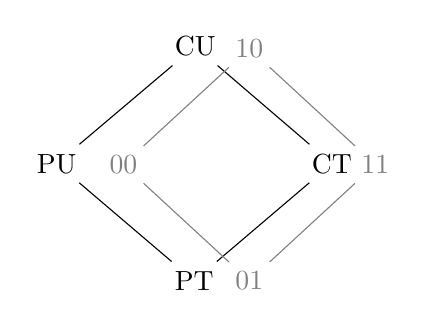
\begin{tikzpicture}
        \begin{scope}
            \node (pt) {\PT};
            \node[above right=of pt] (ct) {\CT}
                edge (pt);
            \node[above left=of pt] (pu) {\PU}
                edge (pt);
            \node[above right=of pu] (cu) {\CU}
                edge (ct)
                edge (pu);
        \end{scope}

        \begin{scope}[xshift=0.7cm,draw=gray,text=gray]
            \node (01) {$ 01 $};
            \node[above right=of 01] (11) {$ 11 $}
                edge (01);
            \node[above left=of 01] (00) {$ 00 $}
                edge (01);
            \node[above right=of 00] (10) {$ 10 $}
                edge (11)
                edge (00);
        \end{scope}
    \end{tikzpicture}
    \caption{Security lattice for SecVerilogBL \cite{Ferraiuolo17} with binary equivalent}
    \label{fig:sec-lattice-bin}
\end{figure}

We define $ \sqcup $ on $ \binSigma $ such that $ \varphi $ is an isomorphism.
This mapping is depicted in figure \ref{fig:sec-lattice-bin}.
Note that public and untrusted correspond to a 0 whereas confidential and trusted correspond to a 1.
This abstraction can be formalized by examining two equivalence-relations or -classes on $ \Sigma $ and $ \binSigma $.
We define two partitionings $ \Sigma/_{\equiv_C} $ and $ \Sigma/_{\equiv_I} $ on $ \Sigma $ which correspond to equivalence classes modulo confidentiality $ \equiv_C $ or modulo integrity respectively $ \equiv_I $.
\begin{align*}
    \Sigma /_{\equiv_C} &= \big\{ \{ \PU, \PT \}, \{ \CU, \CT \} \big\} \\
    \Sigma /_{\equiv_I} &= \big\{ \{ \PU, \CU \}, \{ \PT, \CT \} \big\}
\end{align*}

We coin the names $ \P = [\PU]_{\equiv_C} $, $ \C = [\CU]_{\equiv_C} $, $ \U = [\PU]_{\equiv_I} $ and $ \T = [\PT]_{\equiv_I} $ and lift $ \sqcup $ to be defined on equivalence-classes in the usual fashion, i.e. $ [x] \sqcup [y] = [x \sqcup y] $.
Note, that $ \P \preceq \C $ and $ \T \preceq \U $ with $ \preceq $ again being the partial order inferred from $ \sqcup $ and that it is possible to define $ \sqcup $ solely by working with these equivalence classes:
\begin{equation*}
    \{ x \sqcup y \} = \big(([x]_{\equiv_C} \sqcup [y]_{\equiv_C}) \cap ([x]_{\equiv_I} \sqcup [y]_{\equiv_I}) \big)
\end{equation*}

\begin{example}
    \begin{align*}
        \{ \PU \sqcup \CT \} &= \big(([\PU]_{\equiv_C} \sqcup [\CT]_{\equiv_C}) \cap ([\PU]_{\equiv_I} \sqcup [\CT]_{\equiv_I}) \big) \\
        &= \big((\P \sqcup \C) \cap (\U \sqcup \T) \big) \\
        &= (\C \cap \U) \\
        &= \{ \CU \}
    \end{align*}
\end{example}

This means that labels of the lattice of security labels $ (\Sigma, \sqcup, \sqcap) $ can be tracked by tracking the confidentiality and integrity labels individually.
Dealing with information flow labels in this way also is much more intuitive:
\begin{itemize}
    % TODO: rewrite this
    \item Two sources of information combined are considered to be confidential if \textit{any} of the sources is confidential itself.
    This is sensible as with some result of an operation at least partial information about its confidential source can be inferred if the other public source and the operation are known.
    \item Two sources of information combined are considered to be trustworthy if \textit{both} of the sources are trustworthy themselves.
    This is intuitive as well.
    Non-trustworthy sources of information are assumed to be controlled by an attacker.
    Some piece of information can only be trustworthy if it can be ensured that the attacker does not control it in any way, shape or form.
    This is only given if both of the sources of an operation are not controlled by an attacker, i.e. are trustworthy.
\end{itemize}

The intuition behind $ \sqcup $ as described above perfectly matches $ \binSigma $ as well.
Recall, that \C{} is represented by a 1 and \P{} by a 0 in the binary representation.
That means that two labels $ a = a_Ca_I \in \binSigma $ and $ b = b_Cb_I \in \binSigma $ are in \C{}, i.e. confidential, if $ a $ or $ b $ is confidential, i.e. if \textit{one} of the bits representing the confidentiality of the labels is high, i.e. if $ a_C \lor b_C $.
In turn, these two labels are in $ \T $, i.e. trusted, if $ a $ and $ b $ are trusted, i.e. if \textit{both} of the bits representing the integrity of the labels are high, i.e. if $ a_I \land b_I $.
This allows us to define $ \sqcup $ on $ \binSigma $ again - this time not just semantically:
\begin{equation*}
    a_C a_I \sqcup b_C b_I = (a_C \lor b_C) \cdot (a_I \land b_I)
\end{equation*}

In summary, these paragraphs showed to things:
\begin{enumerate}
    \item Security labels of information can be tracked by using separate labels for the domain of confidentiality and the domain of integrity which in turn can be stored independently of each other.
    This means that the implementation of the MINRV8 architecture does not need to work with the full lattice of information flow labels itself.
    It is sufficient to deal with equivalence classes which can be inferred from individual bits.
    \item The $ \sqcup $ operation on the binary representation of the security labels $ \binSigma $ can be implemented by deriving the confidentiality label by taking the logical disjunction ($ \lor $) of the olds labels and the integrity label by taking the logical conjunction ($ \land $) of the old labels.
\end{enumerate}

This now allows for adding security label tracking to the model whereby the confidentiality and the integrity of values will be tracked.
Labels are assigned on a per bit basis to all values in registers, memory, \glspl{csr} and the cache.
For each variable in the model, an confidentiality or integrity tracking counterpart as (arrays of) unsigned word is added; find an overview of all such variables in table \ref{tbl:ifc-vars}.

\begin{table}
    \centering
    \begin{tabular}{| c | c | c |}
        \hline
        \textbf{Variable} & \textbf{Confidentiality Tracking} & \textbf{Integrity Tracking} \\
        \hline
        {\smv{regs}} & {\smv{regs_conf}} & {\smv{regs_integrity}} \\
        {\smv{memory}} & {\smv{memory_conf}} & {\smv{memory_integrity}} \\
        {\smv{csrs}} & {\smv{\_\_csrs_conf}} & {\smv{\_\_csrs_integrity}} \\
        {\smv{cache.line}} & {\smv{cache.conf}} & {\smv{cache.integrity}} \\
        \hline
    \end{tabular}
    \caption{Information Flow Control Variables}
    \label{tbl:ifc-vars}
\end{table}

These variables transition under the same conditions as their base variable does, e.g. \smv{regs_conf} does a transition if and only if \smv{regs} transitions and \smv{regs_conf} will deduct its content from sources parallel the those of \smv{regs}.
The values themselves change based on the current instruction and its information flow tracking semantics as described in section \ref{sec:ifc-model}.
% TODO: explain why this is the case
The only exception to this is the information flow tracking of the variable \smv{csrs} the labels of which do not change at all.

In other words, the \lstinline[language=SMV,mathescape]{$\dots$_conf} and \lstinline[language=SMV,mathescape]{$\dots$_integrity} variables perfectly mirror the architecture implementation as described in section \ref{sec:model-implementation}.
Rather than simply simulating the MINRV8 architecture in nuXmv, the domain of confidentiality and the domain of integrity of the MINRV8 architecture are tracked in addition to simulating the pure computational-world.

\section{Checking}
\label{sec:checking}

\subsection{Checking \& Refinement Methodology}

\subsection{Checked Properties}

%!TEX root = ../thesis.tex

\section{Results}

This section will cover the results of the verification process as it was described in section \ref{sec:checking}.
The main finding was that there are 8 assumptions which in total grant that the properties as described in section \ref{sec:props} can not be violated, in other words: the MINRV8 architecture models the information flow properties introduced in this thesis, namely \smv{MEMORY_OP_INTEGRITY}, \smv{CSR_INTEGRITY} and \smv{NO_LEAK}, if and only if we assume the 8 assumptions that will be introduced in subsequent sections.

Additionally, roughly 22 bug fix patches\footnote{%
    The number of 22 bug fix patches was measured by counting the amount of patches containing the word \enquote{fix} in its description and being applied to the model file.
} and some \smv{INIT} constraints were applied to the model.
Taken together with aforementioned assumptions these changes to the model mark a fixpoint of the verification process as depicted in figure \ref{fig:ver-process}.

This section is grouped as follows: section \ref{sec:assumptions} will introduce aforementioned assumptions and \smv{INIT} constraints that have been added to the model during the verification process.

Since only assumptions and no architectural refinements were introduced to the model, it was also tested how the model would behave when deliberate breaking points were introduced to it.
These breaking points tried to mimic known vulnerabilities to real-world architectures and will therefore also give an overview of the capabilities of the verification approach of this thesis.
The results to these tests will finally be presented in section \ref{sec:canaries}.

\subsection{Assumptions}
\label{sec:assumptions}

Technically, \smv{INIT} constraints and assumptions serve the same purpose: They limit the state spaces that will be searched for property violations.
Semantically, however, these two concepts should be distinguished in this thesis.
In the model, \smv{INIT} constraints are used to only limit the search of the state space to \textit{valid} counter-examples only.
Validity here means, that properties are not false to begin with and that the initial state of the architecture complies with the specification.

The former aspect of validity is guaranteed by constraining the contents of registers to only contain confidential data when the model starts in machine-mode and to only contain malicious data when the model starts in user-mode.
Furthermore, cache and memory can only contain confidential data if the respective memory region is set to \textit{not} be readable for user-mode and can only contain malicious data if the respective memory region \textit{is} set to be writable by user-mode.
The aforementioned \smv{INIT} constraints simply ensure that the properties to prove are not false upfront.
If, for example, the model would not be constrained to initially only contain confidential data in some register when in machine-mode, nuXmv could find a counter-example violating the \smv{NO_LEAK} property (\ref{itm:prop-no-leak}) where the architecture starts in user-mode and has confidential data in some register trivially violating the respective property.

The latter aspect of validity is guaranteed by two constraints.
The first is rather simple and is depicted in the following snippet:
\begin{lstlisting}[
    language=smv,
    caption={\gls{mstatus} \smv{INIT} constraint for the model}
]
    INIT MIE = 0b_1 -> MPP = 0b_0;
\end{lstlisting}
This constraint ensures that the interrupt handling mechanisms are set up correctly and is mandated by the \gls{riscv} specification (cf. section \ref{sec:rv-exn} and figure \ref{fig:interrupt-handling}).
No other \smv{INIT} constraints are required to set up the initial state of the model correctly and sensibly.
The second constraint sets up caching correctly, i.e. if the cache is valid, it can only point to an address of a region that is cacheable and must match that addresses content unless the respective region is set to be write-back-cacheable.

The 8 assumptions that have been introduced throughout the verification process can be grouped into three categories:
\begin{itemize}
    \item Mode-boundary crossing related assumptions
    \item Memory related assumptions
    \item Memory privilege related assumptions
\end{itemize}

Find an overview of all these assumptions in table \ref{tbl:assumptions-overview}.
Each row represents one assumption and each column one property.
A check mark denotes that the respective assumption is critical for the respective property, i.e. there exists a counter-example proving the property to be false if the assumption at hand is not assumed.
Note that each of the assumptions is critical for at least one property.
This stresses that \enquote{$ \text{assumptions} \Leftrightarrow \text{properties} $} as opposed to \enquote{$ \text{assumptions} \Rightarrow \text{properties} $} since \enquote{$ \neg \text{assumptions} \Rightarrow \neg \text{properties} $}.

\begin{table}
    \centering
    \begin{tabular}{| c r | c | c | c |}
        \multicolumn{1}{r}{} & \multicolumn{1}{r}{} &
        \multicolumn{1}{l}{\tilthdr{\smv{MEMORY_OP_INTEGRITY} (\ref{itm:prop-mem-i})}} &
        \multicolumn{1}{l}{\tilthdr{\smv{CSR_INTEGRITY} (\ref{itm:prop-csr-i})}} &
        \multicolumn{1}{l}{\tilthdr{\smv{NO_LEAK} (\ref{itm:prop-no-leak})}} \\
        \hline % \cline{3-5}
        \multirow{2}{*}{Mode-boundary} & \smv{SAN_ON_CALL} & \checkmark & \checkmark & \\
        \cline{3-5}
        & \smv{CLR_ON_RET} &&& \checkmark \\
        \hline % \cline{3-5}
        \multirow{2}{*}{Memory} & \smv{NO_PUBLIC_READS} & \checkmark & \checkmark & \\
        \cline{3-5}
        & \smv{NO_PUBLIC_WRITES} &&& \checkmark \\
        \hline % \cline{3-5}
        \multirow{4}{*}{Memory privilege} & \smv{SAN_ON_CLASSIFICATION} & \checkmark & \checkmark & \\
        \cline{3-5}
        & \smv{CLR_ON_DECLASSIFICATION} &&& \checkmark \\
        \cline{3-5}
        & \smv{SAN_CACHE_ON_CLASSIFICATION} & \checkmark & \checkmark & \\
        \cline{3-5}
        & \smv{CLR_CACHE_ON_DECLASSIFICATION} &&& \checkmark \\
        \hline % \cline{3-5}
    \end{tabular}
    \caption{Assumptions Compared to Properties}
    \label{tbl:assumptions-overview}
\end{table}

\paragraph{Mode-boundary crossing related assumptions}
The first assumption to be introduced is called \smv{SAN_ON_CALL} and mandates from machine-mode to clear the registers from any untrusted data before continuing to use their contents when entering machine-mode from user-mode.
% TODO: Explain why we had to add this instruction
To allow this, an abstract instruction was added to the model: \minrv{San}, which stands for \textit{sanitize}.
When this instruction is executed, the integrity labels of all registers are set to trusted, i.e. \minrv{1}.
The formal implementation of \smv{SAN_ON_CALL} can be found in snippet \ref{snpt:san-on-call}.

\begin{figure}
    \begin{lstlisting}[
        language=smv,
        caption={Assumption \lstinline{SAN_ON_CALL}},
        label={snpt:san-on-call}
    ]
        G (!priv & X priv -> X op = SAN)
    \end{lstlisting}

    \begin{lstlisting}[
        language=smv,
        caption={Assumption \smv{CLR_ON_RET}},
        label={snpt:clr-on-ret}
    ]
        G (
            priv & X !priv -> regs_conf[0] = 0h_00
                & regs_conf[1] = 0h_00
                & regs_conf[2] = 0h_00
                & regs_conf[3] = 0h_00
        )
    \end{lstlisting}
\end{figure}

Without assuming \smv{SAN_ON_CALL} nuXmv manages to find two counter-examples.
One for property \smv{MEMORY_OP_INTEGRITY} (\ref{itm:prop-mem-i}) and one for \smv{CSR_INTEGRITY} (\ref{itm:prop-csr-i}).
The traces for both counter-examples are depicted in tables \ref{tbl:cex-mem-i-soc} and \ref{tbl:cex-csr-i-soc} respectively.

The format of these tables will be used frequently throughout this thesis to illustrate counter-examples.
To introduce it, table \ref{tbl:cex-mem-i-soc} will be explained in detail now.
Each row of the table represents an instruction being executed and the changes in result of this instruction with the exception of the first row which depicts the processor's initial state.
Whenever a cell is empty, the value represented by it did not change as a result of execution the respective instruction.
Furthermore, the table is separated in three main columns: The first column shows the instructions being executed.
In case of table \ref{tbl:cex-mem-i-soc}, three instructions were executed: \minrv{Ecall}, \minrv{Load} and \minrv{Store}.

The second group of columns hold the information flow labels for the registers and memory on a per-word basis.
During the verification process it was found that no counter-example required information flow labels of a per-bit granularity.
Therefore, for the sake of simplicity, the information flow labels of machine-words in memory or registers were combined to a single label.
The two inner rows in the cells of the second major column denote the labels of the registers (\minrv{r}) and memory (\minrv{m}) respectively whereas the inner columns mark the index of the labels, e.g. in table \ref{tbl:cex-mem-i-soc} all registers and the cells of memory region zero are labelled with \PU{}, i.e. public and untrusted, whereas the cells of memory region one are labelled with \PT{}, i.e. public and trusted, in the initial state.

The third major column shows the status of the processor.
This column is separated into five inner columns as well.
The first (labelled with \minrv{p}) shows the privilege mode of execution where \minrv{U} stands for user-mode and \minrv{M} stands for machine-mode.
The other four columns show the current memory settings per region.
Inner columns starting with \minrv{0} give the settings for first memory region and starting with \minrv{1} for the second memory region respectively.
Inner columns ending with \minrv{c} hold the cacheability settings.
Here, \minrv{UN} stands for uncacheable, \minrv{WB} for write-back-cacheable, \minrv{WT} for write-through-cacheable and \minrv{WP} for write-protected-cacheable (cf. section \ref{sec:minrv8}).
Inner columns ending with \minrv{p} hold the memory privilege settings for the respective region.
Memory privilege settings are indicated by a string of the form:
\begin{grammar}
    <privelege-string> ::= (`-' | `L') (`-' | `R') (`-' | `W')
\end{grammar}

The first letter in the privilege string denotes whether the region is locked (\minrv{L}) or not (\minrv{-}), the second whether user-mode can read the region (\minrv{R}) or not (\minrv{-}) and the third whether user mode can write to the region (\minrv{W}) or not (\minrv{-}).
In table \ref{tbl:cex-mem-i-soc}, none of the regions is locked or cacheable and user mode can write to region zero only and has not further permissions.

Traces generated by nuXmv are infinitely long but finitely representable by including a loop.
In this setting, counter-examples generated by nuXmv always violated the property at hand after having executed the second last instruction whereas the last instruction introduced the loop and led to a fixpoint in the state-space.
For the sake of completeness, the last instruction of counter-example traces will be included nonetheless.

Note that the traces for property \smv{MEMORY_OP_INTEGRITY} in table \ref{tbl:cex-mem-i-soc} and for property \smv{CSR_INTEGRITY} in table \ref{tbl:cex-csr-i-soc} are very similar.
In both traces, the processor starts in user-mode with some untrusted data in the registers.
User-mode then calls machine-mode which decides to use the contents of the registers without sanitization to either write a \gls{csr} or to memory.

The next assumption to be introduced is similar to \smv{SAN_ON_CALL} and is called \smv{CLR_ON_RET}; it says: Whenever machine-mode hands back control to user-mode, the registers must be cleared of any confidential information.
The formal implementation of \smv{CLR_ON_RET} is given in snippet \ref{snpt:clr-on-ret}.
Table \ref{tbl:cex-no-leak-cor} illustrates a counter-example for the \smv{NO_LEAK} (\ref{itm:prop-no-leak}) property when not assuming \smv{CLR_ON_RET} since machine-mode directly hands over confidential data to user-mode by returning control to user-mode without clearing its registers.

\begin{table}
    \begin{subtable}{\textwidth}
        \centering
        \begin{tabular}{| l | r c c c c | c c c c c |}
    \hline
    & & \minrv{0} & \minrv{1} & \minrv{2} & \minrv{3} & \minrv{p} & \minrv{0c} & \minrv{0p} & \minrv{1c} & \minrv{1p} \\
    \hline
    
     & \minrv{r} & \PU & \PU & \PU & \PU & \multirow{2}{*}{\minrv{U}} & \multirow{2}{*}{\minrv{UN}}  & \multirow{2}{*}{\minrv{--W}} & \multirow{2}{*}{\minrv{WB}} & \multirow{2}{*}{\minrv{--W}} \\ & \minrv{m} & \CU & \CU & \CU & \CU &&&&& \\
    \hline
    
    \multirow{2}{*}{\minrv{Ecall}} & \minrv{r} &  &  &  &  & \multirow{2}{*}{\minrv{M}} &   &  &  &  \\ & \minrv{m} &  &  &  &  &&&&& \\
    \hline
    
    \multirow{2}{*}{\minrv{Store 0, 3}} & \minrv{r} &  &  &  &  &  &   &  &  &  \\ & \minrv{m} &  &  &  &  &&&&& \\
    \hline
    
    \multirow{2}{*}{\minrv{Add 2, 1, 0}} & \minrv{r} &  &  &  &  &  &   &  &  &  \\ & \minrv{m} &  &  &  &  &&&&& \\
    \hline
    
\end{tabular}


        \caption{\smv{MEMORY_OP_INTEGRITY} (\ref{itm:prop-mem-i})}
        \label{tbl:cex-mem-i-soc}
    \end{subtable}

    \begin{subtable}{\textwidth}
        \centering
        \begin{tabular}{| l | r c c c c | c c c c c |}
    \hline
    & & \minrv{0} & \minrv{1} & \minrv{2} & \minrv{3} & \minrv{p} & \minrv{0c} & \minrv{0p} & \minrv{1c} & \minrv{1p} \\
    \hline
    
     & \minrv{r} & \PU & \PU & \PU & \PU & \multirow{2}{*}{\minrv{U}} & \multirow{2}{*}{\minrv{UN}}  & \multirow{2}{*}{\minrv{--W}} & \multirow{2}{*}{\minrv{UN}} & \multirow{2}{*}{\minrv{---}} \\ & \minrv{m} & \PU & \PU & \PT & \PT &&&&& \\
    \hline
    
    \multirow{2}{*}{\minrv{Csrrc 1, 0, 1}} & \minrv{r} &  &  &  &  & \multirow{2}{*}{\minrv{M}} &   &  &  &  \\ & \minrv{m} &  &  &  &  &&&&& \\
    \hline
    
    \multirow{2}{*}{\minrv{Csrrs 0, 0, 3}} & \minrv{r} & \CT &  &  &  &  &   &  &  &  \\ & \minrv{m} &  &  &  &  &&&&& \\
    \hline
    
     & \minrv{r} &  &  &  &  &  &   &  &  &  \\ & \minrv{m} &  &  &  &  &&&&& \\
    \hline
    
\end{tabular}


        \caption{\smv{CSR_INTEGRITY} (\ref{itm:prop-csr-i})}
        \label{tbl:cex-csr-i-soc}
    \end{subtable}

    \begin{subtable}{\textwidth}
        \centering
        \begin{tabular}{| l | r c c c c | c c c c c |}
    \hline
    & & \minrv{0} & \minrv{1} & \minrv{2} & \minrv{3} & \minrv{p} & \minrv{0c} & \minrv{0p} & \minrv{1c} & \minrv{1p} \\
    \hline
    
     & \minrv{r} & \CT & \PT & \PT & \PT & \multirow{2}{*}{\minrv{M}} & \multirow{2}{*}{\minrv{UN}}  & \multirow{2}{*}{\minrv{--W}} & \multirow{2}{*}{\minrv{UN}} & \multirow{2}{*}{\minrv{--W}} \\ & \minrv{m} & \PU & \PU & \PU & \PU &&&&& \\
    \hline
    
    \multirow{2}{*}{\minrv{Mret}} & \minrv{r} &  &  &  &  & \multirow{2}{*}{\minrv{U}} &   &  &  &  \\ & \minrv{m} &  &  &  &  &&&&& \\
    \hline
    
    \multirow{2}{*}{\minrv{Load 1, 3}} & \minrv{r} &  &  &  &  &  &   &  &  &  \\ & \minrv{m} &  &  &  &  &&&&& \\
    \hline
    
\end{tabular}


        \caption{\smv{NO_LEAK} (\ref{itm:prop-no-leak})}
        \label{tbl:cex-no-leak-cor}
    \end{subtable}
    \caption{Counter-examples for \smv{SAN_ON_CALL} and \smv{CLR_ON_RET}}
\end{table}

It has already been touched that both assumptions \smv{SAN_ON_CALL} (cf. snippet \ref{snpt:san-on-call}) and \smv{CLR_ON_RET} (cf. snippet \ref{snpt:clr-on-ret}) are similar to each other.
Both were introduced under the label of being \textit{mode-boundary crossing related}, which means that both assumptions are about information flow tracking labels when changing privilege mode - more precisely both are about the labels of register contents.
The relation of these two assumptions, however, also characterizes a pattern that can be recognized for other groups of assumptions as well.
It turned out that for every integrity related assumption such as \smv{SAN_ON_CALL}, there was a similar confidentiality related assumption such as \smv{CLR_ON_RET}.
This can be easily seen in table \ref{tbl:assumptions-overview} where in alternating rows, two groups of assumptions can be distinguished those which are relevant to the properties \smv{MEMORY_OP_INTEGRITY} and \smv{CSR_INTEGRITY} and those which are relevant to the property \smv{NO_LEAK}.
Additionally it is noteworthy that these two groups of assumptions can be characterized by the way they constrain information flow.
Whereas confidentiality related assumptions always constrain flow of information going \textit{out of} machine-mode, integrity related assumptions always constrain flow of information going \textit{into} machine-mode.

\paragraph{Memory related assumptions}
Two assumptions about memory reads and writes join the ranks of these groups, namely \smv{NO_PUBLIC_READS} and \smv{NO_PUBLIC_WRITES} which are formally given in snippet \ref{snpt:no-public-reads} and \ref{snpt:no-public-writes} respectively.
These two assumptions don't express more than the title says; they require machine-mode to never read from or write to public memory.

\begin{figure}
    \begin{lstlisting}[
        language=smv,
        caption={Assumption \lstinline{NO_PUBLIC_READS}},
        label={snpt:no-public-reads}
    ]
        G (priv & op = LOAD -> (
            mem_addr < $REGION0_SIZE
                ? !pmpcfg0.write
                : !pmpcfg1.write
        ))
    \end{lstlisting}

    \begin{lstlisting}[
        language=smv,
        caption={Assumption \lstinline{NO_PUBLIC_WRITES}},
        label={snpt:no-public-writes}
    ]
        G (priv & op = STORE -> (
            mem_addr < $REGION0_SIZE
                ? !pmpcfg0.read
                : !pmpcfg1.read
        ))
    \end{lstlisting}
\end{figure}

The three counter-examples involved in this two assumptions are rather straight-forward as well.
If machine-mode is allowed to load arbitrary words from public memory nuXmv gives a counter-example to the properties \smv{MEMORY_OP_INTEGRITY} (\ref{itm:prop-mem-i}) and \smv{CSR_INTEGRITY} (\ref{itm:prop-csr-i}) where some or all memory is untrusted in the initial state, machine-mode in the next step decides to load some word from an untrusted source in memory and then uses that as target address of a \minrv{Store} instruction or to write a \gls{csr} with.
These counter-examples are illustrated in table \ref{tbl:cex-mem-i-npw} and \ref{tbl:cex-csr-i-npw} respectively.
On the other hand, if machine-mode is allowed to store arbitrary words into public memory, a simple counter-example to the \smv{NO_LEAK} property (\ref{itm:prop-no-leak}) is that machine-mode simply stores a secret into public memory which is then loaded by user-mode as illustrated by the trace in table \ref{tbl:cex-no-leak-npw}.

Additionally, in this counter-example the consequences of assuming \minrv{CLR_ON_RET} can be seen.
Machine-mode tries to hide secrets from user-mode by writing a public value into register zero before returning which is mandated by aforementioned assumption.
Yet, as shown in the last paragraph, this assumption taken alone, does not ensure the absence of \smv{NO_LEAK} related counter-examples.

\begin{table}
    \begin{subtable}{\textwidth}
        \centering
        \begin{tabular}{| l | r c c c c | c c c c c |}
    \hline
    & & \minrv{0} & \minrv{1} & \minrv{2} & \minrv{3} & \minrv{p} & \minrv{0c} & \minrv{0p} & \minrv{1c} & \minrv{1p} \\
    \hline
    
     & \minrv{r} & \CT & \CT & \CT & \CT & \multirow{2}{*}{\minrv{M}} & \multirow{2}{*}{\minrv{UN}}  & \multirow{2}{*}{\minrv{-RW}} & \multirow{2}{*}{\minrv{UN}} & \multirow{2}{*}{\minrv{-RW}} \\ & \minrv{m} & \PU & \PU & \PU & \PU &&&&& \\
    \hline
    
    \multirow{2}{*}{\minrv{Load 0, 3}} & \minrv{r} & \PU &  &  &  &  &   &  &  &  \\ & \minrv{m} &  &  &  &  &&&&& \\
    \hline
    
    \multirow{2}{*}{\minrv{Load 0, 0}} & \minrv{r} &  &  &  &  &  &   &  &  &  \\ & \minrv{m} &  &  &  &  &&&&& \\
    \hline
    
     & \minrv{r} &  &  &  &  &  &   &  &  &  \\ & \minrv{m} &  &  &  &  &&&&& \\
    \hline
    
\end{tabular}


        \caption{\smv{MEMORY_OP_INTEGRITY} (\ref{itm:prop-mem-i})}
        \label{tbl:cex-mem-i-npw}
    \end{subtable}

    \begin{subtable}{\textwidth}
        \centering
        \begin{tabular}{| l | r c c c c | c c c c c |}
    \hline
    & & \minrv{0} & \minrv{1} & \minrv{2} & \minrv{3} & \minrv{p} & \minrv{0c} & \minrv{0p} & \minrv{1c} & \minrv{1p} \\
    \hline
    
     & \minrv{r} & \CT & \CT & \CT & \CT & \multirow{2}{*}{\minrv{M}} & \multirow{2}{*}{\minrv{WB}}  & \multirow{2}{*}{\minrv{-RW}} & \multirow{2}{*}{\minrv{UN}} & \multirow{2}{*}{\minrv{-R-}} \\ & \minrv{m} & \PU & \PU & \PU & \PU &&&&& \\
    \hline
    
    \multirow{2}{*}{\minrv{Load 3, 3}} & \minrv{r} &  &  &  & \PU &  &   &  &  &  \\ & \minrv{m} &  &  &  &  &&&&& \\
    \hline
    
    \multirow{2}{*}{\minrv{Csrrs 2, 3, 3}} & \minrv{r} &  &  &  &  &  &   &  &  &  \\ & \minrv{m} &  &  &  &  &&&&& \\
    \hline
    
    \multirow{2}{*}{\minrv{Mret}} & \minrv{r} &  &  &  &  &  &   &  &  &  \\ & \minrv{m} &  &  &  &  &&&&& \\
    \hline
    
\end{tabular}


        \caption{\smv{CSR_INTEGRITY} (\ref{itm:prop-csr-i})}
        \label{tbl:cex-csr-i-npw}
    \end{subtable}

    \begin{subtable}{\textwidth}
        \centering
        \begin{tabular}{| l | r c c c c | c c c c c |}
    \hline
    & & \minrv{0} & \minrv{1} & \minrv{2} & \minrv{3} & \minrv{p} & \minrv{0c} & \minrv{0p} & \minrv{1c} & \minrv{1p} \\
    \hline
    
     & \minrv{r} & \CT & \PT & \PT & \PT & \multirow{2}{*}{\minrv{M}} & \multirow{2}{*}{\minrv{UN}}  & \multirow{2}{*}{\minrv{LRW}} & \multirow{2}{*}{\minrv{UN}} & \multirow{2}{*}{\minrv{L--}} \\ & \minrv{m} & \PU & \PU & \PT & \PT &&&&& \\
    \hline
    
    \multirow{2}{*}{\minrv{Store 0, 0}} & \minrv{r} &  &  &  &  &  &   &  &  &  \\ & \minrv{m} &  & \CT &  &  &&&&& \\
    \hline
    
    \multirow{2}{*}{\minrv{Csrrc 0, 3, 2}} & \minrv{r} & \PT &  &  &  &  &   &  &  &  \\ & \minrv{m} &  &  &  &  &&&&& \\
    \hline
    
    \multirow{2}{*}{\minrv{Mret}} & \minrv{r} &  &  &  &  & \multirow{2}{*}{\minrv{U}} &   &  &  &  \\ & \minrv{m} &  &  &  &  &&&&& \\
    \hline
    
    \multirow{2}{*}{\minrv{Load 0, 1}} & \minrv{r} & \CT &  &  &  &  &   &  &  &  \\ & \minrv{m} &  &  &  &  &&&&& \\
    \hline
    
    \multirow{2}{*}{\minrv{Load 0, 3}} & \minrv{r} &  &  &  &  &  &   &  &  &  \\ & \minrv{m} &  &  &  &  &&&&& \\
    \hline
    
\end{tabular}


        \caption{\smv{NO_LEAK} (\ref{itm:prop-no-leak})}
        \label{tbl:cex-no-leak-npw}
    \end{subtable}
    \caption{Counter-examples for \smv{NO_PUBLIC_WRITES} and \smv{NO_PUBLIC_READS}}
\end{table}

\paragraph{Memory privilege related assumptions}
The four assumptions that have been introduced up to this point seem to cover all relevant channels of information transmission: registers and memory.
However, these are not enough to ensure that the MINRV8 architecture implements all information flow properties subject to this thesis.
Whereas the two memory related properties covered the group of actions by machine-mode where information directly is given to or taken from user-mode, it is also possible to transmit information indirectly via memory by writing it to or reading it from safe memory regions but doing so while changing the attributes of respective memory regions.
The two assumptions \smv{SANITIZE_ON_DECLASSIFICATION} and \smv{CLR_ON_DECLASSIFICATION} counter issues arising from these vectors.
The former assumption demands from machine-mode to ensure that a memory region does not contain malicious information when its set to be publicly inaccessible.
This assumption is formalized in snippet \ref{snpt:san-on-classify}.
The latter demands from machine-mode to always ensure that a memory region does not contain confidential information when its made publicly accessible.
This assumption is formalized in snippet \ref{snpt:clr-on-declassify}.

\begin{figure}
    \begin{lstlisting}[
        language=smv,
        caption={Assumption \lstinline{SAN_ON_CLASSIFICATION}},
        label={snpt:san-on-classify}
    ]
        G (pmpcfg0.write & X !pmpcfg0.write
            -> memory_integrity[0] = 0h_FF
             & memory_integrity[1] = 0h_FF)
        & G (pmpcfg1.write & X !pmpcfg1.write
            -> memory_integrity[2] = 0h_FF
             & memory_integrity[3] = 0h_FF)
    \end{lstlisting}

    \begin{lstlisting}[
        language=smv,
        caption={Assumption \lstinline{CLR_ON_DECLASSIFICATION}},
        label={snpt:clr-on-declassify}
    ]
        G (!pmpcfg0.read & X pmpcfg0.read
            -> memory_conf[0] = 0h_00
             & memory_conf[1] = 0h_00)
        & G (!pmpcfg1.read & X pmpcfg1.read
            -> memory_conf[2] = 0h_00
             & memory_conf[3] = 0h_00)
    \end{lstlisting}
\end{figure}

The counter-examples when not assuming \smv{SAN_ON_CLASSIFICATION} for properties \smv{MEMORY_OP_INTEGRITY} and \smv{CSR_INTEGRITY} (cf. tables \ref{tbl:cex-csr-i-socl}, \ref{tbl:cex-mem-i-socl}) - as usual - work analogously and illustrate exactly what has been given as intuition for this assumption in the introduction of this paragraph.
In each counter-example, at least one memory region initially is writable for user-mode and contains untrusted data.
Machine-mode changes the privilege settings of that memory region making it non-writable to user-mode and then loads and uses a machine-word which is untrusted violating the respective integrity related property.

The counter-example given when not assuming \smv{CLR_ON_DECLASSIFICATION} is given in table \ref{tbl:cex-no-leak-cod}.
The architecture starts with some confidential data in the memory of the first memory region which is not publicly readable.
In the first step, machine-mode however sets just that memory to being publicly readable.
Machine-mode does clear its registers before giving control back to user-mode, yet this is irrelevant since user-mode can just load the contents from the now accessible memory region one which violates the \smv{NO_LEAK} property (cf. \ref{itm:prop-no-leak}).

\begin{table}
    \begin{subtable}{\textwidth}
        \centering
        \begin{tabular}{| l | r c c c c | c c c c c |}
    \hline
    & & \minrv{0} & \minrv{1} & \minrv{2} & \minrv{3} & \minrv{p} & \minrv{0c} & \minrv{0p} & \minrv{1c} & \minrv{1p} \\
    \hline
    
     & \minrv{r} & \PT & \CT & \PT & \PT & \multirow{2}{*}{\minrv{M}} & \multirow{2}{*}{\minrv{WB}}  & \multirow{2}{*}{\minrv{--W}} & \multirow{2}{*}{\minrv{UN}} & \multirow{2}{*}{\minrv{--W}} \\ & \minrv{m} & \PU & \PU & \PU & \PU &&&&& \\
    \hline
    
    \multirow{2}{*}{\minrv{Csrrc 1, 1, 0}} & \minrv{r} &  & \PT &  &  &  &   & \multirow{2}{*}{\minrv{---}} &  & \multirow{2}{*}{\minrv{---}} \\ & \minrv{m} &  &  &  &  &&&&& \\
    \hline
    
    \multirow{2}{*}{\minrv{Load 2, 0}} & \minrv{r} &  &  & \PU &  &  &   &  &  &  \\ & \minrv{m} &  &  &  &  &&&&& \\
    \hline
    
    \multirow{2}{*}{\minrv{Store 2, 3}} & \minrv{r} &  &  &  &  &  &   &  &  &  \\ & \minrv{m} &  &  &  &  &&&&& \\
    \hline
    
    \multirow{2}{*}{\minrv{Ecall}} & \minrv{r} &  &  &  &  &  &   &  &  &  \\ & \minrv{m} &  &  &  &  &&&&& \\
    \hline
    
\end{tabular}


        \caption{\smv{MEMORY_OP_INTEGRITY} (\ref{itm:prop-mem-i})}
        \label{tbl:cex-mem-i-socl}
    \end{subtable}

    \begin{subtable}{\textwidth}
        \centering
        \begin{tabular}{| l | r c c c c | c c c c c |}
    \hline
    & & \minrv{0} & \minrv{1} & \minrv{2} & \minrv{3} & \minrv{p} & \minrv{0c} & \minrv{0p} & \minrv{1c} & \minrv{1p} \\
    \hline
    
     & \minrv{r} & \CT & \CT & \PT & \PT & \multirow{2}{*}{\minrv{M}} & \multirow{2}{*}{\minrv{UN}}  & \multirow{2}{*}{\minrv{-R-}} & \multirow{2}{*}{\minrv{UN}} & \multirow{2}{*}{\minrv{--W}} \\ & \minrv{m} & \PT & \PT & \CU & \PU &&&&& \\
    \hline
    
    \multirow{2}{*}{\minrv{Csrrc 2, 1, 1}} & \minrv{r} &  &  &  &  &  &   &  &  & \multirow{2}{*}{\minrv{---}} \\ & \minrv{m} &  &  &  &  &&&&& \\
    \hline
    
    \multirow{2}{*}{\minrv{Load 3, 0}} & \minrv{r} &  &  &  & \CU &  &   &  &  &  \\ & \minrv{m} &  &  &  &  &&&&& \\
    \hline
    
    \multirow{2}{*}{\minrv{Csrrs 3, 1, 3}} & \minrv{r} &  &  &  &  &  &   &  &  &  \\ & \minrv{m} &  &  &  &  &&&&& \\
    \hline
    
    \multirow{2}{*}{\minrv{Mret}} & \minrv{r} &  &  &  &  &  &   &  &  &  \\ & \minrv{m} &  &  &  &  &&&&& \\
    \hline
    
\end{tabular}


        \caption{\smv{CSR_INTEGRITY} (\ref{itm:prop-csr-i})}
        \label{tbl:cex-csr-i-socl}
    \end{subtable}

    \begin{subtable}{\textwidth}
        \centering
        \begin{tabular}{| l | r c c c c | c c c c c |}
    \hline
    & & \minrv{0} & \minrv{1} & \minrv{2} & \minrv{3} & \minrv{p} & \minrv{0c} & \minrv{0p} & \minrv{1c} & \minrv{1p} \\
    \hline
    
     & \minrv{r} & \CT & \CT & \CT & \CT & \multirow{2}{*}{\minrv{M}} & \multirow{2}{*}{\minrv{UN}}  & \multirow{2}{*}{\minrv{-R-}} & \multirow{2}{*}{\minrv{UN}} & \multirow{2}{*}{\minrv{---}} \\ & \minrv{m} & \PT & \PT & \CT & \CT &&&&& \\
    \hline
    
    \multirow{2}{*}{\minrv{Csrrs 2, 1, 2}} & \minrv{r} &  &  & \PT &  &  &   &  &  & \multirow{2}{*}{\minrv{-R-}} \\ & \minrv{m} &  &  &  &  &&&&& \\
    \hline
    
    \multirow{2}{*}{\minrv{Clr}} & \minrv{r} & \PT & \PT &  & \PT &  &   &  &  &  \\ & \minrv{m} &  &  &  &  &&&&& \\
    \hline
    
    \multirow{2}{*}{\minrv{Mret}} & \minrv{r} &  &  &  &  & \multirow{2}{*}{\minrv{U}} &   &  &  &  \\ & \minrv{m} &  &  &  &  &&&&& \\
    \hline
    
    \multirow{2}{*}{\minrv{Load 2, 0}} & \minrv{r} &  &  & \CT &  &  &   &  &  &  \\ & \minrv{m} &  &  &  &  &&&&& \\
    \hline
    
    \multirow{2}{*}{\minrv{Slt 2, 3, 0}} & \minrv{r} &  &  & \PT &  &  &   &  &  &  \\ & \minrv{m} &  &  &  &  &&&&& \\
    \hline
    
\end{tabular}


        \caption{\smv{NO_LEAK} (\ref{itm:prop-no-leak})}
        \label{tbl:cex-no-leak-cod}
    \end{subtable}
    \caption{Counter-examples for \smv{CLR_ON_DECLASSIFICATION} and \smv{SAN_ON_CLASSIFICATION}}
\end{table}

Yet, these two assumptions still not suffice to grant the absence of memory privilege related property counter-examples.
It turns out that only ensuring memory regions to not contain confidential/malicious words when (de-)classifying respective regions allows problematic data to remain in cache which bypasses \smv{SAN_ON_CLASSIFICATION} and \smv{CLR_ON_DECLASSIFICATION}.
This brings the need to also assume that the cache is cleared and sanitized by the architecture whenever a memory region is (de-)classified.
This is expressed in the assumptions \smv{SAN_CACHE_ON_CLASSIFICATION} and \smv{CLR_CACHE_ON_DECLASSFICATION} (cf. snippets \ref{snpt:sanc-on-classify}, \ref{snpt:clrc-on-declassify}).

\begin{figure}
    \begin{lstlisting}[
        language=smv,
        caption={Assumption \lstinline{SAN_CACHE_ON_CLASSIFICATION}},
        label={snpt:sanc-on-classify}
    ]
        G (pmpcfg0.write & X !pmpcfg0.write
                & cache.valid & cache.addr < $REGION0_SIZE
            -> cache.integrity = 0h_FF) &
        G (pmpcfg1.write & X !pmpcfg1.write
                & cache.valid & $REGION0_SIZE <= cache.addr
            -> cache.integrity = 0h_FF)
    \end{lstlisting}

    \begin{lstlisting}[
        language=smv,
        caption={Assumption \lstinline{CLR_CACHE_ON_DECLASSIFICATION}},
        label={snpt:clrc-on-declassify}
    ]
        G (!pmpcfg0.read & X pmpcfg0.read
                & cache.valid & cache.addr < $REGION0_SIZE
            -> cache.conf = 0h_00) &
        G (!pmpcfg1.read & X pmpcfg1.read
                & cache.valid & $REGION0_SIZE <= cache.addr
            -> cache.conf = 0h_00)
    \end{lstlisting}
\end{figure}

This time around, the counter-examples given by nuXmv are not completely straight forward.
As a start, consider the counter-examples generated when not assuming \smv{SAN_CACHE_ON_DECLASSFICATION} for the \smv{MEMORY_OP_INTEGRITY} property in table \ref{tbl:cex-mem-i-scocl}.
In the first instruction, machine-mode sets memory region one to be inaccessible by user-mode which does not violate assumption \minrv{SAN_ON_CLASSIFICATION} since all memory provides trusted values.
In the next instruction, machine-mode decides to load a word from memory which happens to be untrusted.
This must come from cache since no other memory cell matches this label.
This is only possible because memory region one is set to be write-back-cacheable where writes not necessarily must be reflect in memory.
This word is then used as address for a \minrv{Load} instruction violating property \ref{itm:prop-mem-i}.
The counter-example for property \smv{CSR_INTEGRITY} (\ref{itm:prop-csr-i}) depicted in table \ref{tbl:cex-csr-i-scocl} follows the same pattern and therefore will not be handled separately in this context.

The trace generated to prove the \smv{NO_LEAK} property (\ref{itm:prop-no-leak}) wrong when not assuming \minrv{CLR_CACHE_ON_DECLASSIFICATION} flips the integrity related counter-examples.
It is given in table \ref{tbl:cex-no-leak-ccod}.
Here, memory region zero is set to be write-back-cacheable.
This time though, machine-mode declassifies it in the first instruction as opposed to the previous counter-examples where the respective region was being classified.
Machine-mode then gives back control to user-mode which performs a load.
Again, a mysterious confidential word appears in register three which must have come from the cache of memory region one since only this region is accessible to user-mode.

\begin{table}
    \begin{subtable}{\textwidth}
        \centering
        \begin{tabular}{| l | r c c c c | c c c c c |}
    \hline
    & & \minrv{0} & \minrv{1} & \minrv{2} & \minrv{3} & \minrv{p} & \minrv{0c} & \minrv{0p} & \minrv{1c} & \minrv{1p} \\
    \hline
    
     & \minrv{r} & \CT & \CT & \CT & \CT & \multirow{2}{*}{\minrv{M}} & \multirow{2}{*}{\minrv{WB}}  & \multirow{2}{*}{\minrv{---}} & \multirow{2}{*}{\minrv{UN}} & \multirow{2}{*}{\minrv{L-W}} \\ & \minrv{m} & \CT & \CT & \CT & \CT &&&&& \\
    \hline
    
    \multirow{2}{*}{\minrv{Csrrs 0, 1, 0}} & \minrv{r} & \PT &  &  &  &  &   & \multirow{2}{*}{\minrv{--W}} &  &  \\ & \minrv{m} &  &  &  &  &&&&& \\
    \hline
    
    \multirow{2}{*}{\minrv{Clr}} & \minrv{r} &  & \PT & \PT & \PT &  &   &  &  &  \\ & \minrv{m} &  &  &  &  &&&&& \\
    \hline
    
    \multirow{2}{*}{\minrv{Mret}} & \minrv{r} &  &  &  &  & \multirow{2}{*}{\minrv{U}} &   &  &  &  \\ & \minrv{m} &  &  &  &  &&&&& \\
    \hline
    
    \multirow{2}{*}{\minrv{Loadi 1 IMM}} & \minrv{r} &  & \PU &  &  &  &   &  &  &  \\ & \minrv{m} &  &  &  &  &&&&& \\
    \hline
    
    \multirow{2}{*}{\minrv{Store 0, 1}} & \minrv{r} &  &  &  &  &  &   &  &  &  \\ & \minrv{m} &  &  &  &  &&&&& \\
    \hline
    
    \multirow{2}{*}{\minrv{Clr}} & \minrv{r} &  &  &  &  & \multirow{2}{*}{\minrv{M}} &   &  &  &  \\ & \minrv{m} &  &  &  &  &&&&& \\
    \hline
    
    \multirow{2}{*}{\minrv{San}} & \minrv{r} &  & \PT &  &  &  &   &  &  &  \\ & \minrv{m} &  &  &  &  &&&&& \\
    \hline
    
    \multirow{2}{*}{\minrv{Csrrc 0, 3, 0}} & \minrv{r} &  &  &  &  &  &   & \multirow{2}{*}{\minrv{---}} &  &  \\ & \minrv{m} &  &  &  &  &&&&& \\
    \hline
    
    \multirow{2}{*}{\minrv{Load 1, 1}} & \minrv{r} &  & \PU &  &  &  &   &  &  &  \\ & \minrv{m} &  &  &  &  &&&&& \\
    \hline
    
    \multirow{2}{*}{\minrv{Store 1, 2}} & \minrv{r} &  &  &  &  &  &   &  &  &  \\ & \minrv{m} &  &  &  &  &&&&& \\
    \hline
    
     & \minrv{r} &  &  &  &  &  &   &  &  &  \\ & \minrv{m} &  &  &  &  &&&&& \\
    \hline
    
\end{tabular}


        \caption{\smv{MEMORY_OP_INTEGRITY} (\ref{itm:prop-mem-i})}
        \label{tbl:cex-mem-i-scocl}
    \end{subtable}

    \begin{subtable}{\textwidth}
        \centering
        \begin{tabular}{| l | r c c c c | c c c c c |}
    \hline
    & & \minrv{0} & \minrv{1} & \minrv{2} & \minrv{3} & \minrv{p} & \minrv{0c} & \minrv{0p} & \minrv{1c} & \minrv{1p} \\
    \hline
    
     & \minrv{r} & \CT & \CT & \CT & \CT & \multirow{2}{*}{\minrv{M}} & \multirow{2}{*}{\minrv{WB}}  & \multirow{2}{*}{\minrv{---}} & \multirow{2}{*}{\minrv{UN}} & \multirow{2}{*}{\minrv{---}} \\ & \minrv{m} & \CT & \CT & \CT & \CT &&&&& \\
    \hline
    
    \multirow{2}{*}{\minrv{Csrrs 1, 1, 3}} & \minrv{r} &  & \PT &  &  &  &   & \multirow{2}{*}{\minrv{--W}} &  &  \\ & \minrv{m} &  &  &  &  &&&&& \\
    \hline
    
    \multirow{2}{*}{\minrv{Clr}} & \minrv{r} & \PT &  & \PT & \PT &  &   &  &  &  \\ & \minrv{m} &  &  &  &  &&&&& \\
    \hline
    
    \multirow{2}{*}{\minrv{Mret}} & \minrv{r} &  &  &  &  & \multirow{2}{*}{\minrv{U}} &   &  &  &  \\ & \minrv{m} &  &  &  &  &&&&& \\
    \hline
    
    \multirow{2}{*}{\minrv{Loadi 2 IMM}} & \minrv{r} &  &  & \PU &  &  &   &  &  &  \\ & \minrv{m} &  &  &  &  &&&&& \\
    \hline
    
    \multirow{2}{*}{\minrv{Store 0, 2}} & \minrv{r} &  &  &  &  &  &   &  &  &  \\ & \minrv{m} &  &  &  &  &&&&& \\
    \hline
    
    \multirow{2}{*}{\minrv{Clr}} & \minrv{r} &  &  &  &  & \multirow{2}{*}{\minrv{M}} &   &  &  &  \\ & \minrv{m} &  &  &  &  &&&&& \\
    \hline
    
    \multirow{2}{*}{\minrv{San}} & \minrv{r} &  &  & \PT &  &  &   &  &  &  \\ & \minrv{m} &  &  &  &  &&&&& \\
    \hline
    
    \multirow{2}{*}{\minrv{Csrrc 0, 3, 0}} & \minrv{r} &  &  &  &  &  &   & \multirow{2}{*}{\minrv{---}} &  &  \\ & \minrv{m} &  &  &  &  &&&&& \\
    \hline
    
    \multirow{2}{*}{\minrv{Load 0, 1}} & \minrv{r} & \PU &  &  &  &  &   &  &  &  \\ & \minrv{m} &  &  &  &  &&&&& \\
    \hline
    
    \multirow{2}{*}{\minrv{Csrrs 1, 3, 0}} & \minrv{r} &  &  &  &  &  &   &  &  & \multirow{2}{*}{\minrv{--W}} \\ & \minrv{m} &  &  &  &  &&&&& \\
    \hline
    
    \multirow{2}{*}{\minrv{Csrrc 2, 3, 1}} & \minrv{r} &  &  &  &  &  &   &  &  & \multirow{2}{*}{\minrv{---}} \\ & \minrv{m} &  &  &  &  &&&&& \\
    \hline
    
\end{tabular}


        \caption{\smv{CSR_INTEGRITY} (\ref{itm:prop-csr-i})}
        \label{tbl:cex-csr-i-scocl}
    \end{subtable}

    \begin{subtable}{\textwidth}
        \centering
        \begin{tabular}{| l | r c c c c | c c c c c |}
    \hline
    & & \minrv{0} & \minrv{1} & \minrv{2} & \minrv{3} & \minrv{p} & \minrv{0c} & \minrv{0p} & \minrv{1c} & \minrv{1p} \\
    \hline
    
     & \minrv{r} & \PT & \CT & \PT & \PT & \multirow{2}{*}{\minrv{M}} & \multirow{2}{*}{\minrv{UN}}  & \multirow{2}{*}{\minrv{L--}} & \multirow{2}{*}{\minrv{WB}} & \multirow{2}{*}{\minrv{--W}} \\ & \minrv{m} & \PT & \PT & \PU & \PU &&&&& \\
    \hline
    
    \multirow{2}{*}{\minrv{Csrrs 1, 1, 3}} & \minrv{r} &  & \PT &  &  &  &   &  &  & \multirow{2}{*}{\minrv{-RW}} \\ & \minrv{m} &  &  &  &  &&&&& \\
    \hline
    
    \multirow{2}{*}{\minrv{Mret}} & \minrv{r} &  &  &  &  & \multirow{2}{*}{\minrv{U}} &   &  &  &  \\ & \minrv{m} &  &  &  &  &&&&& \\
    \hline
    
    \multirow{2}{*}{\minrv{Load 3, 0}} & \minrv{r} &  &  &  & \CU &  &   &  &  &  \\ & \minrv{m} &  &  &  &  &&&&& \\
    \hline
    
    \multirow{2}{*}{\minrv{Mov 0, 0}} & \minrv{r} &  &  &  &  &  &   &  &  &  \\ & \minrv{m} &  &  &  &  &&&&& \\
    \hline
    
\end{tabular}


        \caption{\smv{NO_LEAK} (\ref{itm:prop-no-leak})}
        \label{tbl:cex-no-leak-ccod}
    \end{subtable}
    \caption{Counter-examples for \smv{CLR_CACHE_ON_DECLASSIFICATION} and \smv{SAN_CACHE_ON_CLASSIFICATION}}
\end{table}

\subsection{Canaries}
\label{sec:canaries}

% TODO: Introduce Intel x86 architecture
In this section, it will be presented how the model of the MINRV8 architecture was altered in order to implement real-world attacks to the Intel x86 architecture.
By default, the MINRV8 architecture was not vulnerable to these attacks, however, making the architecture vulnerable will put the approach of this thesis to formally verify an instruction set architecture to a test.

\subsubsection{Cache Poisoning Attack on x86}

The - as it will be called here - cache poisoning attack was discovered and presented by Rafal Wojtczuk and Joanna Rutkowska in their publication \textit{Attacking SMM Memory via Intel\textsuperscript{\textregistered} CPU Cache Poisoning} \cite{Wojtczuk09}.
The term \enquote{SMM memory} refers to a specific region of memory that is designed to be only accessible by the mode of highest privilege in x86 architectures: System Management Mode.
This memory should be written only on start-up and then locked down for later write-accesses.
Wojtczuk and Rutkowska, however, managed to find a vulnerability to the x86 architecture which allowed them to effectively write to SMM memory without SMM privileges by marking respective memory region as write-back-cacheable.
The attack comprises the following steps and requires administrator privileges on the machine to be attacked:
\begin{enumerate}
    \item Mark SMM memory as write-back-cacheable using administrator privileges
    \item \label{itm:cache-pois-mem}
    Generate write accesses to the memory.
    Since the region is marked as write-back-cacheable, the writes will not be propagated to the memory controller which would drop these accesses but will be cached.
    \item \label{itm:cache-pois-smi}
    Trigger an System Management Interrupt to transfer control to System Management Mode.
    Depending on the specific addresses written System Management Mode will now execute code written with administrator privileges.
\end{enumerate}

Steps \ref{itm:cache-pois-mem} and \ref{itm:cache-pois-smi} can also be swapped.
If instead of a write access the cache is read in this case, this attack vector can then be utilized to read SMM memory.

This attack does not fully apply to the MINRV8 architecture since it does not support as fine grained privilege modes.
However, the basic idea can still be implemented if the following changes are made to the model:
\begin{itemize}
    \item For all cache transition relations, do not check whether current privilege mode suffices for the memory operation at hand
    \item For load accesses to memory, do not check whether current privilege mode suffices for the memory read if the address is being cached
\end{itemize}

These changes manage to introduce a vulnerability to the MINRV8 architecture.
If assuming all assumptions introduced in section \ref{sec:assumptions}, nuXmv manages to find a counter-example for all three information flow properties.
These are depicted in table \ref{tbl:cex-cache-vuln}.
As usual, the traces for \smv{MEMORY_OP_INTEGRITY} (\ref{itm:prop-mem-i}) and \smv{CSR_INTEGRITY} (\ref{itm:prop-csr-i}) as depicted in tables \ref{tbl:cex-mem-i-cache-vuln} and \ref{tbl:cex-csr-i-cache-vuln} are highly similar.
In both cases, the user-mode initially executes a \minrv{Store} instruction which is not reflected in memory.
The changes are written to cache-only and therefore must target memory region one since this is set to be write-back cacheable.
Here, it can be clearly seen that dropping memory privilege controls on cache-writes and -reads leads to certain states which are inconsistent with the MINRV8 specification since memory region one is locked and as neither the read- nor the write- bit is set, both user- and machine-mode should not be able to read from or write to memory region one.
Yet, the cache-access succeeds.

In the next step, a pending external interrupt is taken which leads to the transition to machine-mode.
Machine-mode sanitizes the input registers and performs a load instruction targeting the same address as the user's store instruction.
Which leads to an untrusted value being stored in register two.
This value is then used to perform a load or store operation.
In the case of the original cache-poisoning attack, the authors wrote to executable memory directly influencing what would be executed by System Management Mode.
Since the MINRV8 model does not support a model of executable memory, it is not possible to implement this exact vulnerability.
However, these counter-examples show that it is still possible to implement the very core of the cache poisoning attack into the MINRV8 model which leads to a similar vulnerability in the architecture.

This carries over to the counter-example for property \smv{NO_LEAK} (\ref{itm:prop-no-leak}) which is depicted in table \ref{tbl:cex-no-leak-cache-vuln}.
This counter-example more closely matches the alternative version of the cache-poisoning attack used for reading SMM memory.
nuXmv sets the initial state up such that the cache holds some confidential data for one of the memory regions which both are set to be write-back-cacheable and non-readable to user-mode.
Yet still, user-mode can gain access to the confidential word in cache as no access controls are performed when reading from cache.

One distinction from the original cache-poisoning attack to these counter-examples is that here the attacker does need need to set the attacked memory region to be cacheable in the first place.
This difference does not play a major role since the attack can take place nonetheless if some memory region happens to be locked down to user-mode and is set to be write-back-cacheable, still this weakens the attack to some degree.

What can be done to mitigate this attack?
Obviously, the vulnerability purposefully introduced to the architecture could be dropped.
It is not clear, though, how realistic this characteristic of the MINRV8 architecture is since at least in the case of the x86 architecture, the findings of \cite{Wojtczuk09} suggest that is not possible for the hardware to perform privilege checks when writing to the cache.
Therefore this vulnerability stresses a weakness of the model as implemented in this thesis.
Since the MINRV8 architecture only knows two privilege modes, the problem of setting potentially \enquote{interesting} regions of memory to be cacheable for an attack does not come into play.
If, however, three or more privilege modes were given the question would arise which of the non-user-modes should be able to set caching methods for memory regions.
If for example the supervisor-mode of \gls{riscv} also was part of the MINRV8 architecture and additionally would be allowed to write \gls{pmacfg} registers, a possible attack vector to gain access to machine-mode would be to first gain access to supervisor-mode and then set memory regions of interest to be write-back-cacheable.

One possible approach to this would be to extend the MINRV8 architecture by said supervisor-mode and to test how architectural measures could mitigate this vulnerability, if for hardware-reasons, the platform could not check privileges for cache accesses.

\begin{table}
    \begin{subtable}{\textwidth}
        \centering
        \begin{tabular}{| l | r c c c c | c c c c c |}
    \hline
    & & \minrv{0} & \minrv{1} & \minrv{2} & \minrv{3} & \minrv{p} & \minrv{0c} & \minrv{0p} & \minrv{1c} & \minrv{1p} \\
    \hline
    
     & \minrv{r} & \PU & \PU & \PU & \PU & \multirow{2}{*}{\minrv{U}} & \multirow{2}{*}{\minrv{UN}}  & \multirow{2}{*}{\minrv{L--}} & \multirow{2}{*}{\minrv{WB}} & \multirow{2}{*}{\minrv{L--}} \\ & \minrv{m} & \PT & \PT & \PT & \PT &&&&& \\
    \hline
    
    \multirow{2}{*}{\minrv{Store 2, 0}} & \minrv{r} &  &  &  &  &  &   &  &  &  \\ & \minrv{m} &  &  &  &  &&&&& \\
    \hline
    
     & \minrv{r} &  &  &  &  & \multirow{2}{*}{\minrv{M}} &   &  &  &  \\ & \minrv{m} &  &  &  &  &&&&& \\
    \hline
    
    \multirow{2}{*}{\minrv{San}} & \minrv{r} & \PT & \PT & \PT & \PT &  &   &  &  &  \\ & \minrv{m} &  &  &  &  &&&&& \\
    \hline
    
    \multirow{2}{*}{\minrv{Load 2, 2}} & \minrv{r} &  &  & \PU &  &  &   &  &  &  \\ & \minrv{m} &  &  &  &  &&&&& \\
    \hline
    
    \multirow{2}{*}{\minrv{Load 0, 2}} & \minrv{r} &  &  &  &  &  &   &  &  &  \\ & \minrv{m} &  &  &  &  &&&&& \\
    \hline
    
    \multirow{2}{*}{\minrv{Or 0, 1, 2}} & \minrv{r} &  &  &  &  &  &   &  &  &  \\ & \minrv{m} &  &  &  &  &&&&& \\
    \hline
    
\end{tabular}


        \caption{\smv{MEMORY_OP_INTEGRITY} (\ref{itm:prop-mem-i})}
        \label{tbl:cex-mem-i-cache-vuln}
    \end{subtable}

    \begin{subtable}{\textwidth}
        \centering
        \begin{tabular}{| l | r c c c c | c c c c c |}
    \hline
    & & \minrv{0} & \minrv{1} & \minrv{2} & \minrv{3} & \minrv{p} & \minrv{0c} & \minrv{0p} & \minrv{1c} & \minrv{1p} \\
    \hline
    
     & \minrv{r} & \PU & \PU & \PU & \PU & \multirow{2}{*}{\minrv{U}} & \multirow{2}{*}{\minrv{UN}}  & \multirow{2}{*}{\minrv{-R-}} & \multirow{2}{*}{\minrv{WB}} & \multirow{2}{*}{\minrv{L--}} \\ & \minrv{m} & \PT & \PT & \PT & \PT &&&&& \\
    \hline
    
    \multirow{2}{*}{\minrv{Store 0, 2}} & \minrv{r} &  &  &  &  &  &   &  &  &  \\ & \minrv{m} &  &  &  &  &&&&& \\
    \hline
    
    \multirow{2}{*}{\minrv{Slt 2, 0, 0}} & \minrv{r} &  &  &  &  & \multirow{2}{*}{\minrv{M}} &   &  &  &  \\ & \minrv{m} &  &  &  &  &&&&& \\
    \hline
    
    \multirow{2}{*}{\minrv{San}} & \minrv{r} & \PT & \PT & \PT & \PT &  &   &  &  &  \\ & \minrv{m} &  &  &  &  &&&&& \\
    \hline
    
    \multirow{2}{*}{\minrv{Load 2, 0}} & \minrv{r} &  &  & \PU &  &  &   &  &  &  \\ & \minrv{m} &  &  &  &  &&&&& \\
    \hline
    
    \multirow{2}{*}{\minrv{Csrrc 1, 0, 2}} & \minrv{r} &  & \CT &  &  &  &   &  & \multirow{2}{*}{\minrv{UN}} &  \\ & \minrv{m} &  &  &  & \PU &&&&& \\
    \hline
    
    \multirow{2}{*}{\minrv{Csrrc 3, 3, 2}} & \minrv{r} &  &  &  &  &  &   &  &  &  \\ & \minrv{m} &  &  &  &  &&&&& \\
    \hline
    
\end{tabular}


        \caption{\smv{CSR_INTEGRITY} (\ref{itm:prop-csr-i})}
        \label{tbl:cex-csr-i-cache-vuln}
    \end{subtable}

    \begin{subtable}{\textwidth}
        \centering
        \begin{tabular}{| l | r c c c c | c c c c c |}
    \hline
    & & \minrv{0} & \minrv{1} & \minrv{2} & \minrv{3} & \minrv{p} & \minrv{0c} & \minrv{0p} & \minrv{1c} & \minrv{1p} \\
    \hline
    
     & \minrv{r} & \PU & \PU & \PU & \PU & \multirow{2}{*}{\minrv{U}} & \multirow{2}{*}{\minrv{WB}}  & \multirow{2}{*}{\minrv{--W}} & \multirow{2}{*}{\minrv{WB}} & \multirow{2}{*}{\minrv{--W}} \\ & \minrv{m} & \PU & \PU & \PU & \PU &&&&& \\
    \hline
    
    \multirow{2}{*}{\minrv{Load 1, 0}} & \minrv{r} &  & \CU &  &  &  &   &  &  &  \\ & \minrv{m} &  &  &  &  &&&&& \\
    \hline
    
    \multirow{2}{*}{\minrv{Loadi 0 IMM}} & \minrv{r} &  &  &  &  &  &   &  &  &  \\ & \minrv{m} &  &  &  &  &&&&& \\
    \hline
    
\end{tabular}


        \caption{\smv{NO_LEAK} (\ref{itm:prop-no-leak})}
        \label{tbl:cex-no-leak-cache-vuln}
    \end{subtable}
    \caption{Counter-examples for the Cache Vulnerability}
    \label{tbl:cex-cache-vuln}
\end{table}

\subsection{Limitations}

%!TEX root = ../thesis.tex

\section{Conclusion}
\label{sec:conclusion}

Find an overview of this thesis as a whole in figure \ref{fig:overview}.
As a first step, the MINRV8 architecture inspired by the RISC-V architecture was defined and implemented in nuXmv in section \ref{sec:minrv8}.
In sections \ref{sec:ifc}-\ref{sec:checking}, we developed information flow semantics and three information flow properties forming an information flow policy in spirit of the work of \citeauthor{Ferraiuolo17} \cite{Ferraiuolo17}.
The information flow semantics were used to augmented the model of the MINRV8 by information flow tracking.
In section \ref{sec:results} we introduced eight assumptions that, when implemented software running in machine-mode such as \glspl{os}, guarantee the absence of vulnerabilities covered by aforementioned information flow properties.
We evaluated our model, the properties and the assumptions by showing that taken together, they manage to detect both the cache poisoning \cite{Wojtczuk09} and the SYSRET vulnerability \cite{Dunlap19}.
Finally in section \ref{sec:discussion}, we discussed the limitations and the scope of our work and reflected whether our methodology is trustworthy.

\begin{figure}
    \centering
    \includegraphics[width=\textwidth]{figures/thesis-overview.png}
    \caption{Thesis Overview}
    \label{fig:overview}
\end{figure}

In the introduction, we set three other goals: it was claimed that the approach presented as part of this thesis is \textit{viable}, i.e. feasible, realistic and generalizable, \textit{relevant}, i.e. it is able to detect issues, and \textit{supplemental}, i.e. it enhances on related work.

We were able to show the the implementation of the MINRV8 architecture models the property \enquote{assumptions $ \Leftrightarrow $ properties}.
This was put to a test by showing that said implementation does violate the properties of section \ref{sec:checking} when it is exposed to the cache poisoning or SYSRET vulnerability.
In other words: it was shown that the three properties \smv{MEMORY_OP_INTEGRITY}, \smv{CSR_INTEGRITY} and \smv{NO_LEAK} cover at least vulnerabilities related to the cache poisoning or SYSRET vulnerability.
This marks the main result of this thesis and shows that this work is \textit{relevant}.
Furthermore, mitigations to these vulnerabilities can be verified using the same model.
It must be decided on a case by case basis whether a given violation of the information flow policy actually marks a vulnerability of the architecture leaving it with the need to be altered or marks a feature the risks of which must be controlled in software.
To achieve this, a novel approach of using model checking for verifying architectural specifications was used.
We discussed another case where model checking was applied to architectural specifications in \ref{sec:related-model-checking} \cite{BradfieldS16}.
However, this approach was flawed, did not use model checking to its full potential and implemented a very limited model
In \cite{BradfieldS16}, the properties only took one transition in the state spaces into consideration whereas in this work we proved properties touching traces of possibly infinite length.
Additionally, in \cite{BradfieldS16}, the model only comprised instructions related to mode-transitioning whereas here, we implemented a more or less complete set of basic \gls{risc} instructions.
This, taken together with the discussion of other related work in section \ref{sec:related-work} shows that this work is \textit{supplemental}.

What is left to show is that this work is \textit{viable}.
All proofs were run on a laptop equipped with an Intel Core i7-7500U CPU with 8GB of RAM.
It is safe to say, that these are very moderate hardware requirements.
Proofs were conducted per property.
None of these proofs took more than 60s.
While we can give no clear count of working hours spent on this thesis, all of it was developed and written by a single person in no more than eight months.
During this time, this person did not solely work on this thesis.
In a non-research scenario one can assume that development would be more straight forward since it would not include the definition of an architecture.
Due to the exponential blow-up of binary encoded state spaces, there are no guarantees that this approach scales well to realistic and complete architectures.
However, there are two reasons which make seem likely that this approach does indeed scale.
Firstly, the proofs here were ran on a small machine and didn't take much time.
\todo{Strenghtened by related work, i.e. IFT in OS track by one label only}
Secondly, in section \ref{sec:discuss-observations} it was discussed that bit-wise tracking of information flow might be dropped, i.e. there is room for performance improvements.
All of this gives good reasons to believe that our approach is indeed \textit{viable} and could be applied to other architectures with reasonable effort.

\todo[inline]{Bridge}

In section \ref{sec:verify-spec} four design goals were discussed that were initially introduced in \cite{Reid17}.
These were defined to apply to high level properties for specifications and list as follows:
\begin{displaycquote}[pp.88:2-3]{Reid17}
    The central design challenge we face is to create a set of properties that:
    \begin{itemize}
        \item express the major guarantees that programmers depend on;
        \item are concise so that architects can easily review and remember the entire set of properties;
        \item are stable so that architectural extensions don't invalidate large numbers of rules;
        \item and that describe the architecture differently from existing specification to reduce the risk of common-mode failure.
    \end{itemize}
\end{displaycquote}

These objectives are met by our work:
\begin{itemize}
    \item The assumptions guarantee programmers of \glspl{os} and compilers that programs adhering to these do not violate basic information flow properties.
    \item Both assumptions and properties are small in number and short and can be expressed in intuitive natural language, hence concise.
    \item The properties itself are completely architecture independent and as such stable.
    The assumptions are architecture dependent and rely on both instructions available and concrete semantics of these instructions.
    However, we feel subjectively that only basic mechanics are used and predict that the assumptions in a practical environment of an architecture subject to change should be relatively stable as well.
    \item The premise of information flow tracking on specification level is to describe the architecture from a different point of view.
    It is therefore obvious that there is very little risk of common-mode failure.
\end{itemize}

Finally, we give an outlook on future work:
\begin{description}
    \item[Executable memory] First and foremost, the model could be enhanced by a model of executable memory to more closely resemble modern architectures.
    This was discussed extensively in section \ref{sec:discuss-arch}.
    \item[MMU] In light of \cite{KhakpourSD13} a model of an \gls{mmu} could be implemented to make use of information flow tracking on user-mode level.
    This was discussed in section \ref{sec:related-work}.
    \item[Machine-generated model] The model of the architecture that was implemented by hand in this thesis could be generated from existing machine-readable architectural specifications.
    For example, there are machine-readable versions of the ARM architecture; both \cite{Reid17,Fox02} either used or developed machine-readable specifications that might be used for this endeavor.
    For RISC-V, there also is a formal specification available \cite{RiscvSpecFormal}.
    Not implementing the model by hand would \begin{enumerate*}[label=\alph*)]
        \item possibly enhance the trust in the model itself, depending on the trust in the source and the translation procedure, and
        \item make the approach even more viable and stable towards architectural changes.
    \end{enumerate*}
    \item[Complete model] An obvious improvement of this work would be to enhance it by more instructions and use a bigger word-size.
    This would bring the model closer to real-world architectures but might also introduce performance issues.
    \item[Verification of assumptions] Finally, it could be investigated whether the assumptions introduced in context of the verification process serve as practical and sensible target of verification for compilers and/or \glspl{os}.
    It could be investigated whether code generated from compilers or \glspl{os} itself adheres to these assumptions.
    Applying the assumptions to the next level of abstraction in modern computing might lead to more easy and mainstream usage of formal verification in programming.
    Since these properties are stable for a given architecture, there could be off the shelf tools verifying programs for high-level correctness removing the need to tailor verification efforts per system to be verified.
\end{description}

\todo[inline]{Final summary}


\bibliography{references}
\bibliographystyle{alpha}

\end{document}
